\chapter{Sistema Proposto}\label{cap3_proposta}

{ O sistema proposto consiste em um \textit{soft-core} da \textit{ISA RISC-V}
    de 32 \textit{bits} com as extensões \textbf{I}, \textbf{M} e \textbf{F},
    podendo ser sintetizado nas versões \textbf{RV32I}, \textbf{RV32IM} ou
    \textbf{RV32IMF}. A extensão \textbf{Zicsr} com os Registradores de Controle
    e Estado (\textit{CSR}) é parcialmente implementada em todas as três
    configurações. Chamadas de sistema (\textit{syscalls}) também são implementadas.
}

{ Cada uma das combinações da \textit{ISA} pode ser realizada em três
    microarquiteturas diferentes: unicicilo, multiciclo ou \textit{pipeline} de
    cinco estágios. Assim, o processador pode ser sintetizado em nove
    combinações diferentes.
}

{ O projeto utiliza a placa de desenvolvimento \textit{terasIC DE1-SoC} contendo
    diversos periféricos e um \textit{SoC Intel Altera Cyclone-V}. A maioria dos
    periféricos presentes na plataforma tem controladores implementados com
    Entradas e Saídas Mapeadas em Memória (\textit{MMIO}) para que o
    \textit{soft-core} possa utilizá-los. A síntese dos controladores dos
    periféricos, como a saída de vídeo, entrada de teclado e barramento
    \textit{RS-232} é opcional.
}

\section{Organização do projeto}
    { O projeto é organizado seguindo o seguinte arranjo de pastas:
    }
\begin{verbatim}
    ┌─ core                     (arquivos que implementam o soft-core)
    │  ├─ clock                 (arquivos de interface e controle de sinais
    │  │                            de clock do processador)
    │  ├─ memory                (arquivos de interface/controle de memória)
    │  ├─ misc                  (módulos como somador e multiplexador de
    │  │                            largura definidas por parâmetros)
    │  ├─ peripherals           (interfaces e controladores para os
    │  │                            periféricos da FPGA)
    │  ├─ risc_v                (projeto do processador RISC-V)
    │  │  ├─ CPU.v              (arquivo top-level do processador)
    │  │  ├─ Control_*.v        (módulos de controle de cada microarquitetura)
    │  │  ├─ Datapath_*.v       (módulos do caminho de dados de cada µarch)
    │  │  └─ ...                (demais módulos do processador)
    │  ├─ config.v              (arquivo de configuração de versão do
    │  │                            processador a implementar, seus
    │  │                            periféricos e endereçamento de memória
    │  │                            das interfaces MMIO)
    │  ├─ default_data.mif      (arquivo de inicialização de memória de
    │  │                            dados usado na síntese do projeto)
    │  ├─ default_framebuffer.mif   (arquivo de inicialização de memória de
    │  │                                vídeo usada na síntese do projeto)
    │  ├─ default_text.mif      (arquivo de inicialização de memória de
    │  │                            texto usado na síntese do projeto)
    │  ├─ fpga_top.sdc          (restrições desejadas de temporização do
    │  │                            sistema sintetizado)
    │  └─ fpga_top.v            (interface verilog entre o soft-core e a
    │                               placa de desenvolvimento)
    ├─ doc                      (documentação e guias do projeto)
    ├─ project                  (arquivos de projeto do Quartus)
    │  ├─ de1_soc
    │  │  ├─ db                 (arquivos de saída intermediários do
    │  │  │                         Quartus; pasta ignorada pelo git)
    │  │  ├─ incremental_db     (arquivos de saída intermediários do
    │  │  │                         Quartus; pasta ignorada pelo git)
    │  │  ├─ output_files       (arquivos de saída do Quartus; os logs de
    │  │  │                         síntese gerados pelo script "make.sh"
    │  │  │                         ficam aqui, bem como o .sof da última
    │  │  │                         síntese completa; ignorada pelo git)
    │  │  ├─ fpga_top.qpf       (arquivo de projeto do Quartus indicando
    │  │  │                         a versão do projeto)
    │  │  ├─ fpga_top.qsf       (arquivo de projeto do Quartus contendo
    │  │  │                         as configurações do projeto)
    │  │  └─ ...                (outros arquivos de projeto do Quartus)
    │  └─ ...                   (outros modelos de FPGA)
    ├─ system                   (códigos em assembly RISC-V implementando
    │                               as chamadas de sistema e macros)
    ├─ test
    │  ├─ assembly_testbench    (códigos em assembly RISC-V para testar o
    │  │                            funcionamento correto das instruções
    │  │                            do processador)
    │  ├─ gtkwave               (formas de onda predefinidas para visualizar
    │  │                            os arquivos .vcd gerados pelo ModelSim
    │  │                            usando o GTKwave)
    │  ├─ mif_library           (testbenches assembly compilados para o
    │  │                            formato .mif para gravação na memória
    │  │                            da FPGA)
    │  ├─ simulation            (arquivos de saída da simulação pelo
    │  │                            ModelSim; pasta ignorada pelo git)
    │  ├─ simulation_scripts    (scripts .do para que o ModelSim simule o
    │  │                            sistema corretamente)
    │  ├─ sof_library           (arquivos .sof das versões do processador
    │  │                            prontos para gravação na FPGA)
    │  └─ verilog_testbench     (testbench usado para simular as entradas
    │                               da FPGA, inicializá-la e definir o
    │                               tempo de simulação)
    ├─ tools
    │  ├─ bitmap_converter      (conversor de imagens para uso na FPGA)
    │  ├─ rars                  (montador e simulador de assembly RISC-V)
    │  └─ riscv-disassembler    (disassembler de instruções usado para
    │                               traduzir o código de máquina dos
    │                               sinais de instruções no GTKWave e
    │                               como ferramenta de linha de comando)
    ├─ vendor
    │  └─ ...                   (licenças dos softwares utilizados)
    ├─ inst_decode.sh           (script para traduzir de forma rápida uma
    │                               instrução em formato hexadecimal
    │                               usando o riscv-disassembler)
    ├─ LICENSE                  (licença do sistema implementado)
    ├─ make.sh                  (script para síntese e simulação de todas
    │                               as variantes do processador)
    ├─ gtkwave.sh               (script para invocar o GTKWave usando a
    │                               pasta do projeto como diretório raíz;
    │                               necessita do GTKWave instalado)
    ├─ rars.sh                  (script para invocar o RARS presente em
    │                               tools/rars usando a pasta do projeto
    │                               como diretório raiz; necessita do
    │                               Java instalado)
    └─ README.md                (README sobre o que é o projeto e como
                                    utilizá-lo)
\end{verbatim}


    { O trabalho também é organizado de forma a facilitar a migração para placas de
        desenvolvimento diferentes da \textit{DE1-SoC} ou trocar o \textit{soft-core}
        desenvolvido por outra implementação, independente da sua \textit{ISA}.
        O \textit{soft-core} implementado se encontra no caminho
        \texttt{core/risc\_v}. Assim, os demais módulos presentes na pasta \texttt{core}
        não dependem da arquitetura do processador, exceto a tela de
        \textit{debug} presente na interface de vídeo, que mostra os nomes dos
        registradores segundo as convenções da \textit{RISC-V}. No entanto, a tela de
        \textit{debug} foi projetada de modo a ser relativamente fácil
        customizá-la para utilização em outra arquitetura.
    }

    { A Figura~\ref{fig:diagram_fpga_blocks} mostra um diagrama de blocos simplificado
        da hierarquia dos módulos que compõe o projeto sintetizável. A principal
        estrutura, a \texttt{fpga\_top} representa a placa de desenvolvimento, enquanto
        a \texttt{cpu} é o \textit{soft-core} implementado.
    }

    \begin{figure}[H]
    \centering
        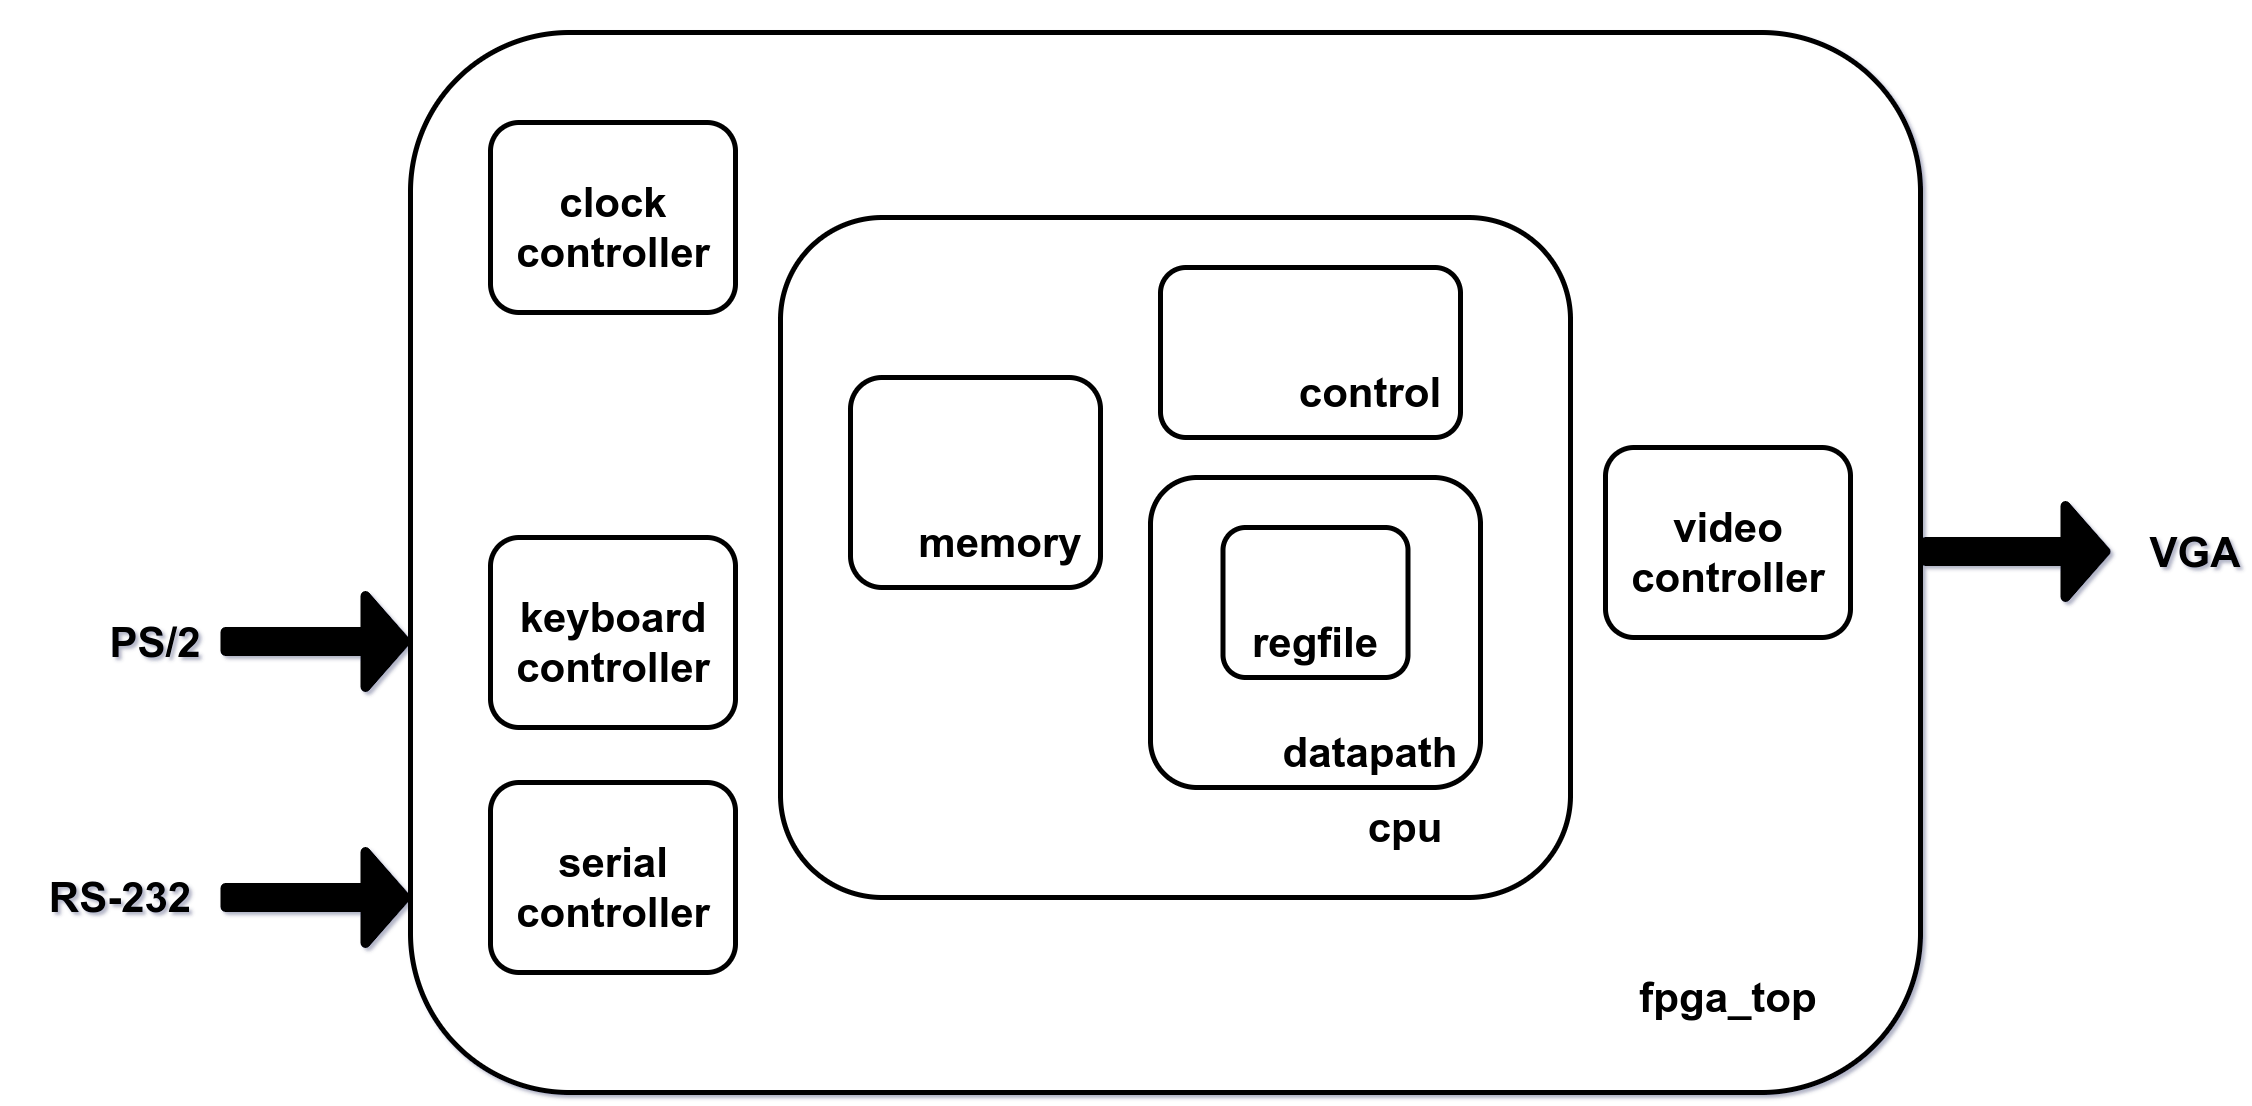
\includegraphics[width=0.9\linewidth]{../images/fpga/fpga_simplified_block_diagram.png}
        \caption{Diagrama de blocos simplificado do sistema}\label{fig:diagram_fpga_blocks}
    \end{figure}

    {
        O arquivo \texttt{core/config.v} possui todas as opções de configuração,
        definição de parâmetros e endereçamento de memória dos módulos, facilitando
        escolher as extensões, microarquitetura e periféricos sintetizados. Outras
        pastas e arquivos relevantes serão discutidos nas próximas seções.
    }


\section{Implementação dos \textit{soft-cores} (Incompleto)}
    { Todos os \textit{soft-cores} implementados possuem execução em ordem, sem
        \textit{branch prediction}, sem \textit{caching} de memória e sem
        \textit{Return Address Stack}. O processador é escalar e possui um
        único \textit{hart}. Como a implementação atual só utiliza blocos de
        memória presentes no chip da FPGA, sem utilizar as memórias
        \textit{SRAM} e \textit{DRAM} externas presentes na placa de
        desenvolvimento, e também não faz uso de memória secundária, as operações
        de \textit{load} e \textit{store} transferem dados diretamente entre os
        registradores e os blocos de memória \textit{M10K}.
    }

    \subsection{Microarquitetura Uniciclo (Incompleto)}

        { Os processsadores uniciclo com extensões I e IM são implementados
            conforme o diagrama da Figura~\ref{fig:diagram_rv32i_uni}. O módulo
            de controle é implementado somente com lógica combinacional, e a
            frequência máxima de operação é limitada pela instrução mais lenta
            do processador.
        }

        \begin{figure}[H]
        \centering
            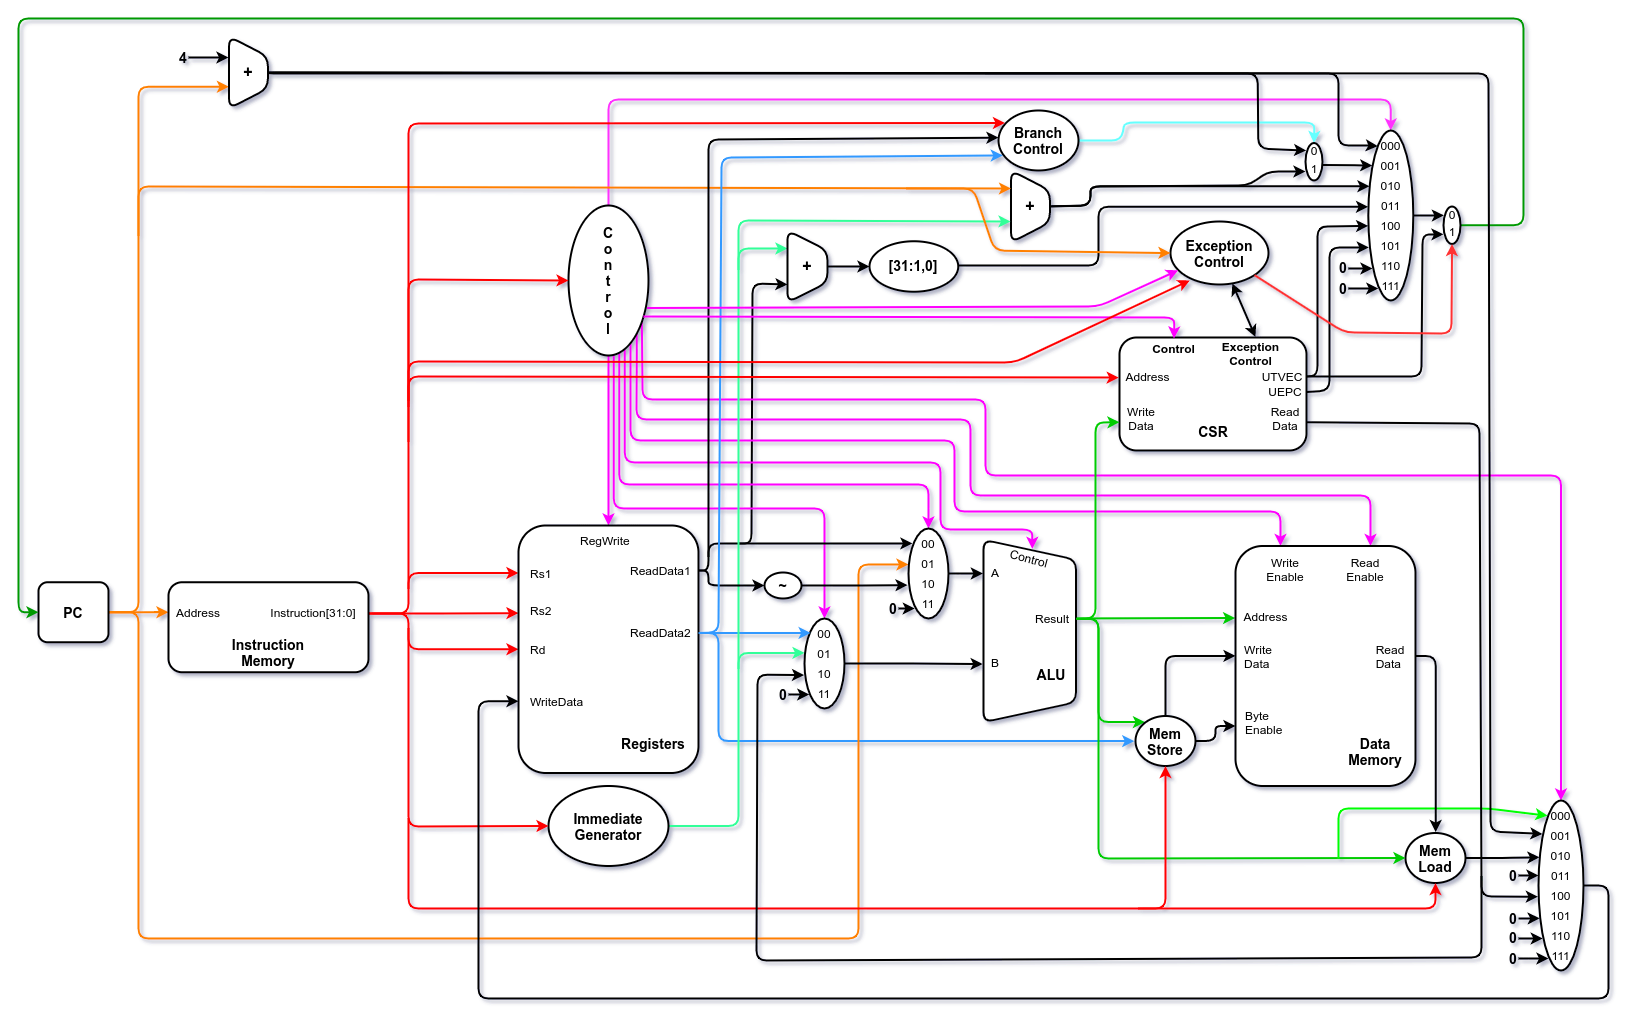
\includegraphics[width=.9\linewidth]{../images/uarch_diagrams/singlecycle-RV32I-RV32IM.png}
            \caption{Diagrama da implementação das \textit{ISAs} RV32I e RV32IM na
            microarquitetura uniciclo}\label{fig:diagram_rv32i_uni}
        \end{figure}

        { O processador uniciclo com extensão IMF é implementado conforme o
            diagrama da Figura~\ref{fig:diagram_rv32imf_uni}. A unidade lógica e
            aritmética de ponto flutuante utiliza uma frequência de \textit{clock}
            maior que a do resto do processador, e é o único módulo da implementação
            uniciclo que utiliza mais de um ciclo de relógio para realizar sua
            operação. A frequência máxima de operação do \textit{clock} principal
            do processador continua limitada pela operação mais lenta.
        }

        \begin{figure}[H]
        \centering
            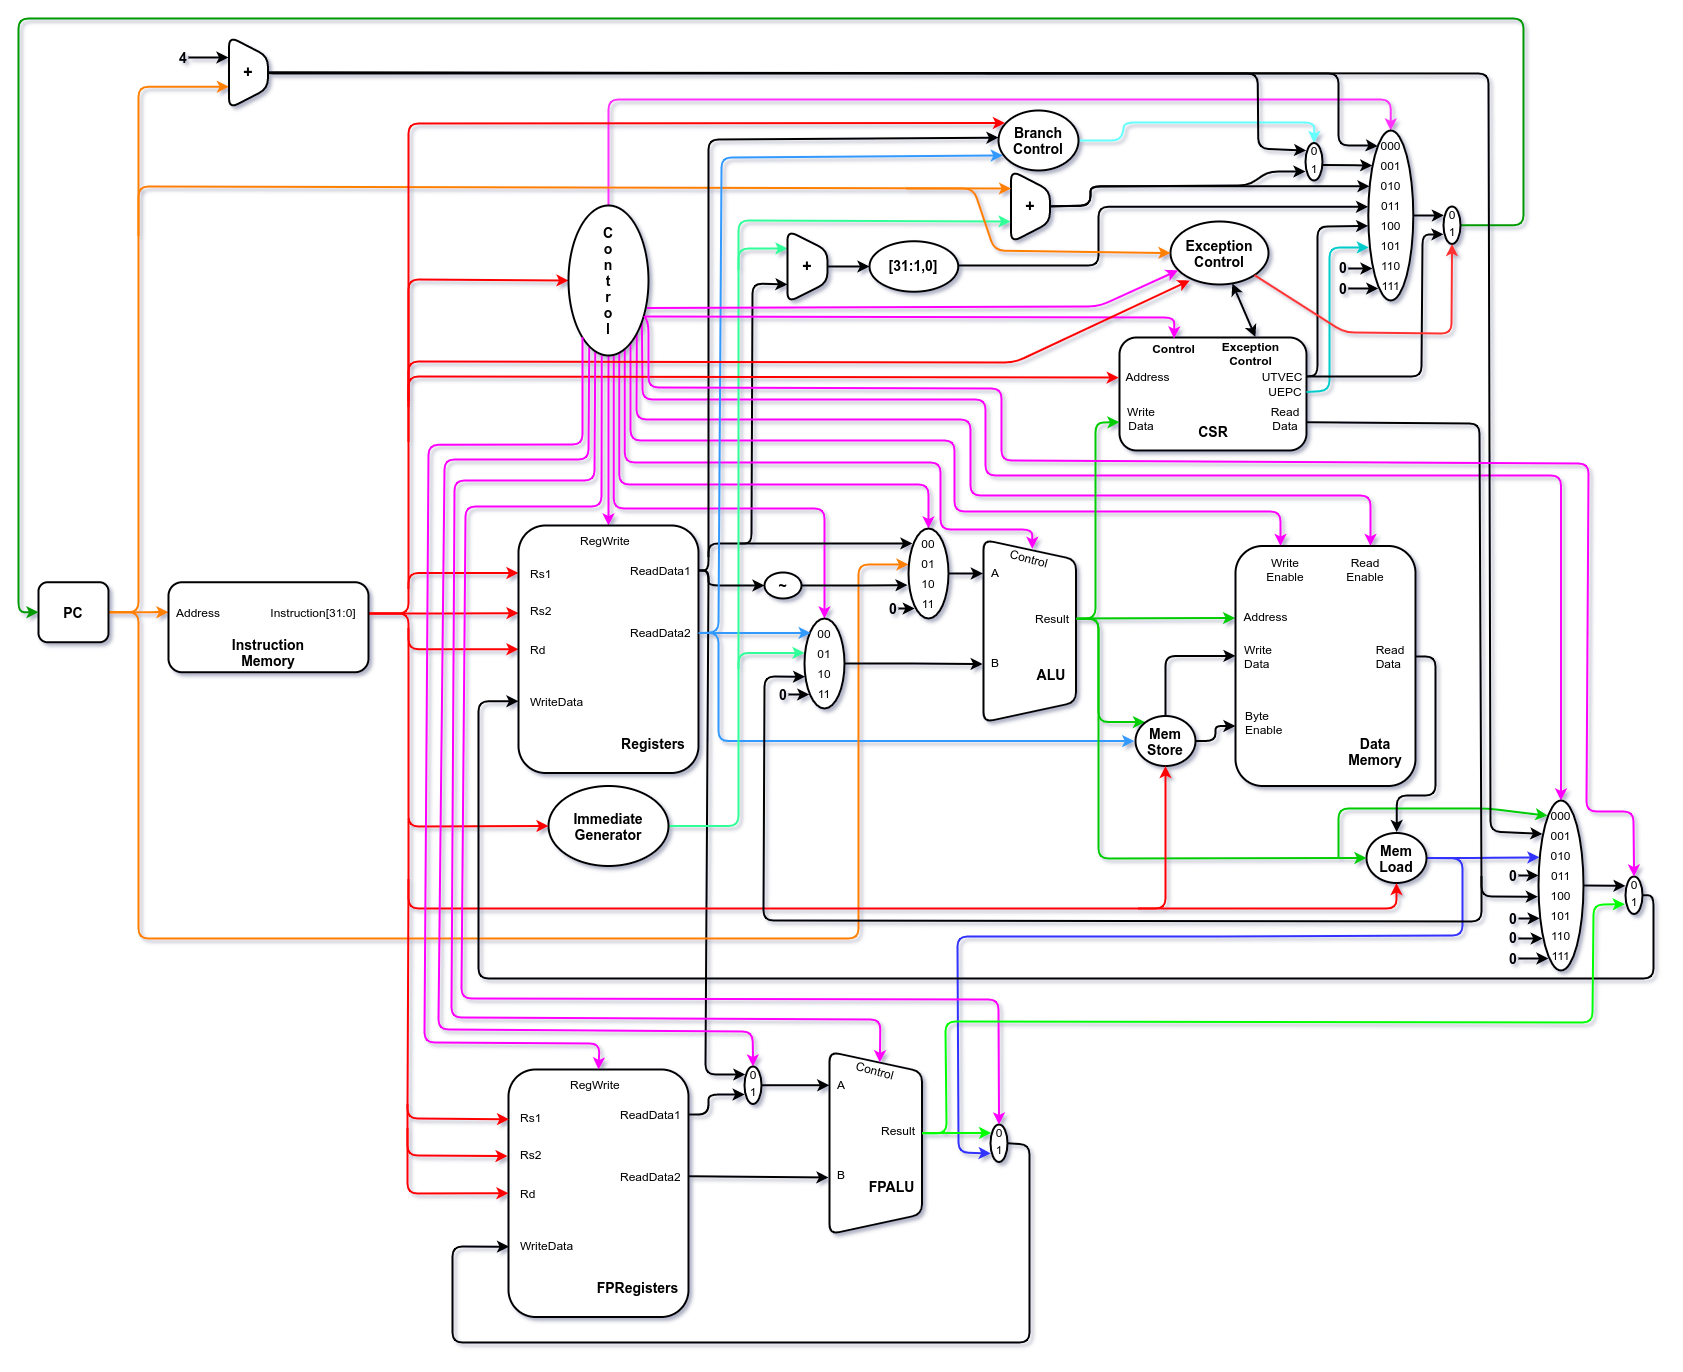
\includegraphics[width=.9\linewidth]{../images/uarch_diagrams/singlecycle-RV32IMF.png}
            \caption{Diagrama da implementação da \textit{ISA} RV32IMF na
            microarquitetura uniciclo}\label{fig:diagram_rv32imf_uni}
        \end{figure}

    \subsection{Microarquitetura Multiciclo (Incompleto)}
        { Os processadores multiciclo com extensões I e IM são implementados
            conforme o diagrama da Figura~\ref{fig:diagram_rv32i_multi}. A
            unidade de controle é implementada utilizando microcódigo para
            executar as instruções. Com isso, a frequência de operação do
            processador depende da operação mais lenta do microcódigo, e não da
            execução da instrução completa.
        }

        \begin{figure}[H]
        \centering
            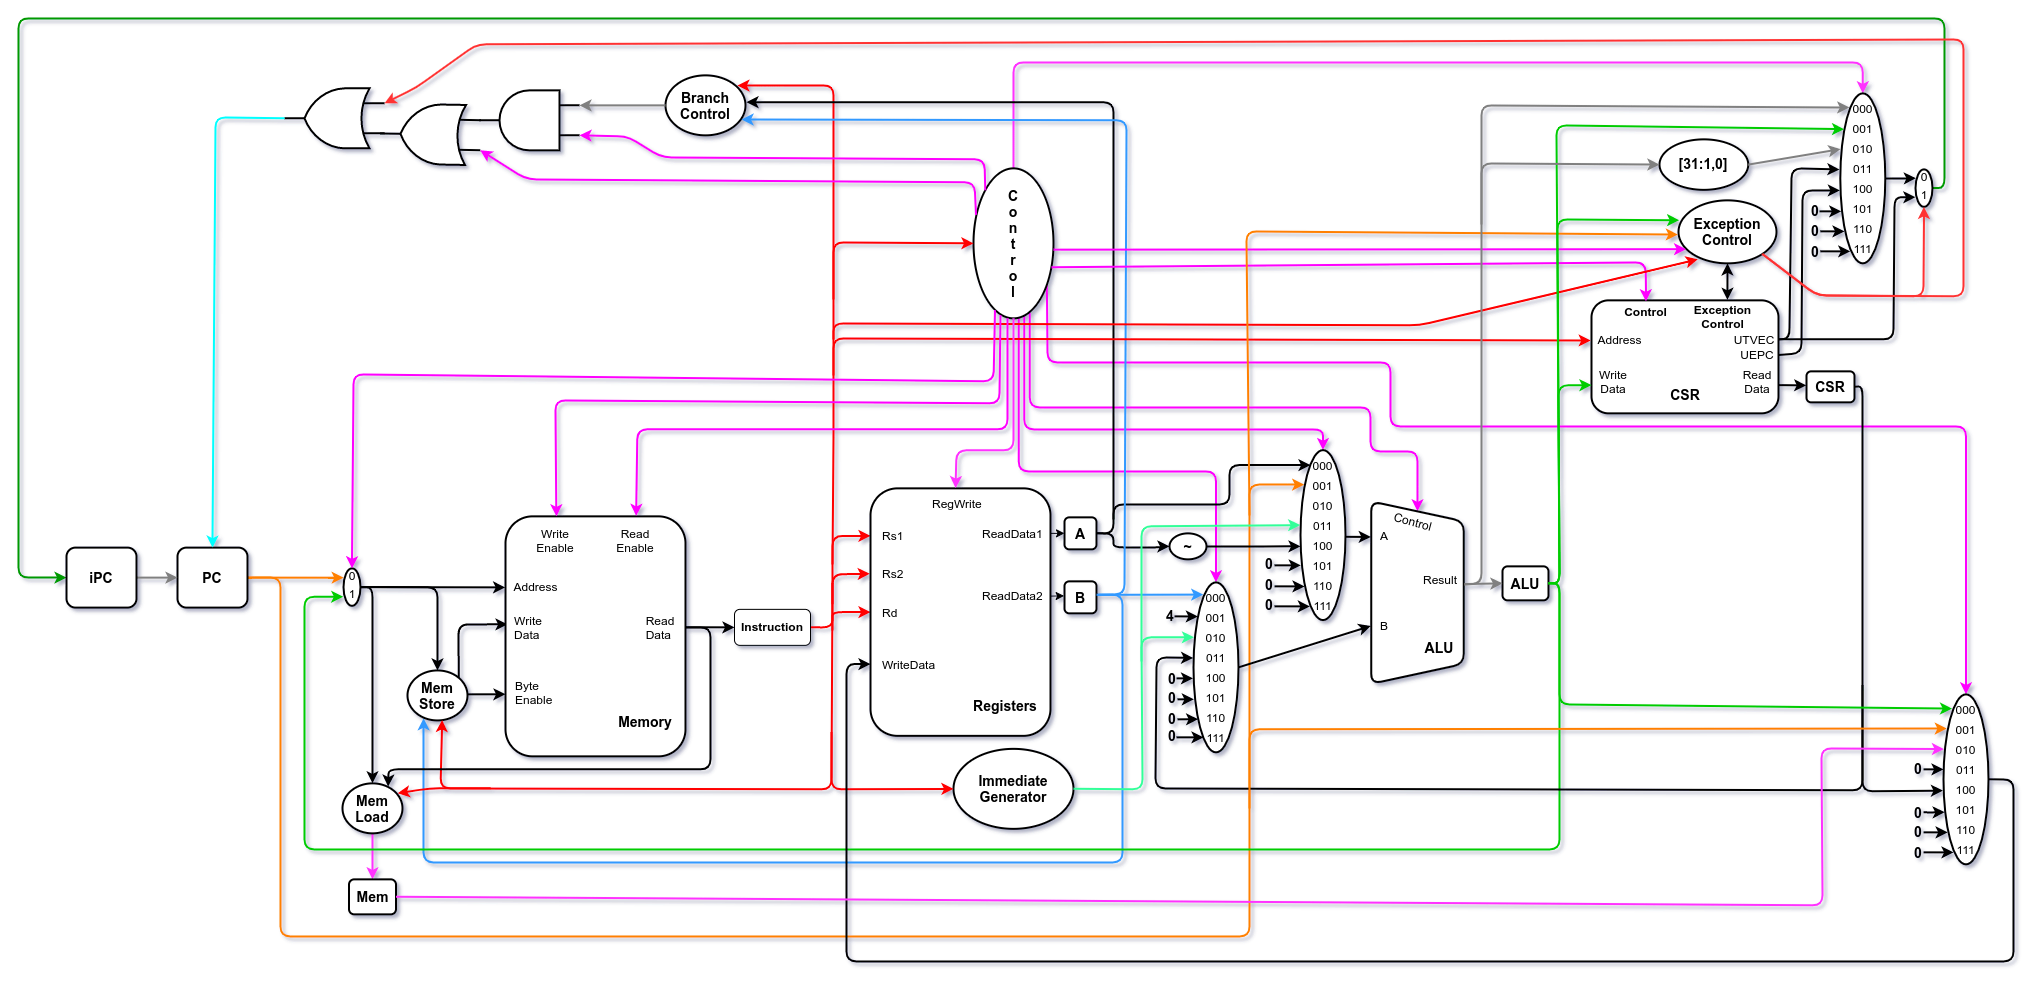
\includegraphics[width=.9\linewidth]{../images/uarch_diagrams/multicycle-RV32I-RV32IM.png}
            \caption{Diagrama da implementação das \textit{ISAs} RV32I e RV32IM na
            microarquitetura multiciclo}\label{fig:diagram_rv32i_multi}
        \end{figure}

        { O processador multicilo com extensões IMF é implementado conforme o
            diagrama da Figura~\ref{fig:diagram_rv32imf_multi}. A unidade lógica
            e aritmética de ponto flutuante utiliza uma frequência de \textit{clock}
            mais alta que a do resto do processador, e possui um sinal de
            \textit{ready} que causa o \textit{stall} do clock principal do
            processador enquanto a operação de ponto flutuante não completa.
            Assim, a frequência do \textit{clock} do processador é variável, já
            que em operações de ponto flutuante o ciclo do relógio é mais longo
            que em outras operações.
        }

        \begin{figure}[H]
        \centering
            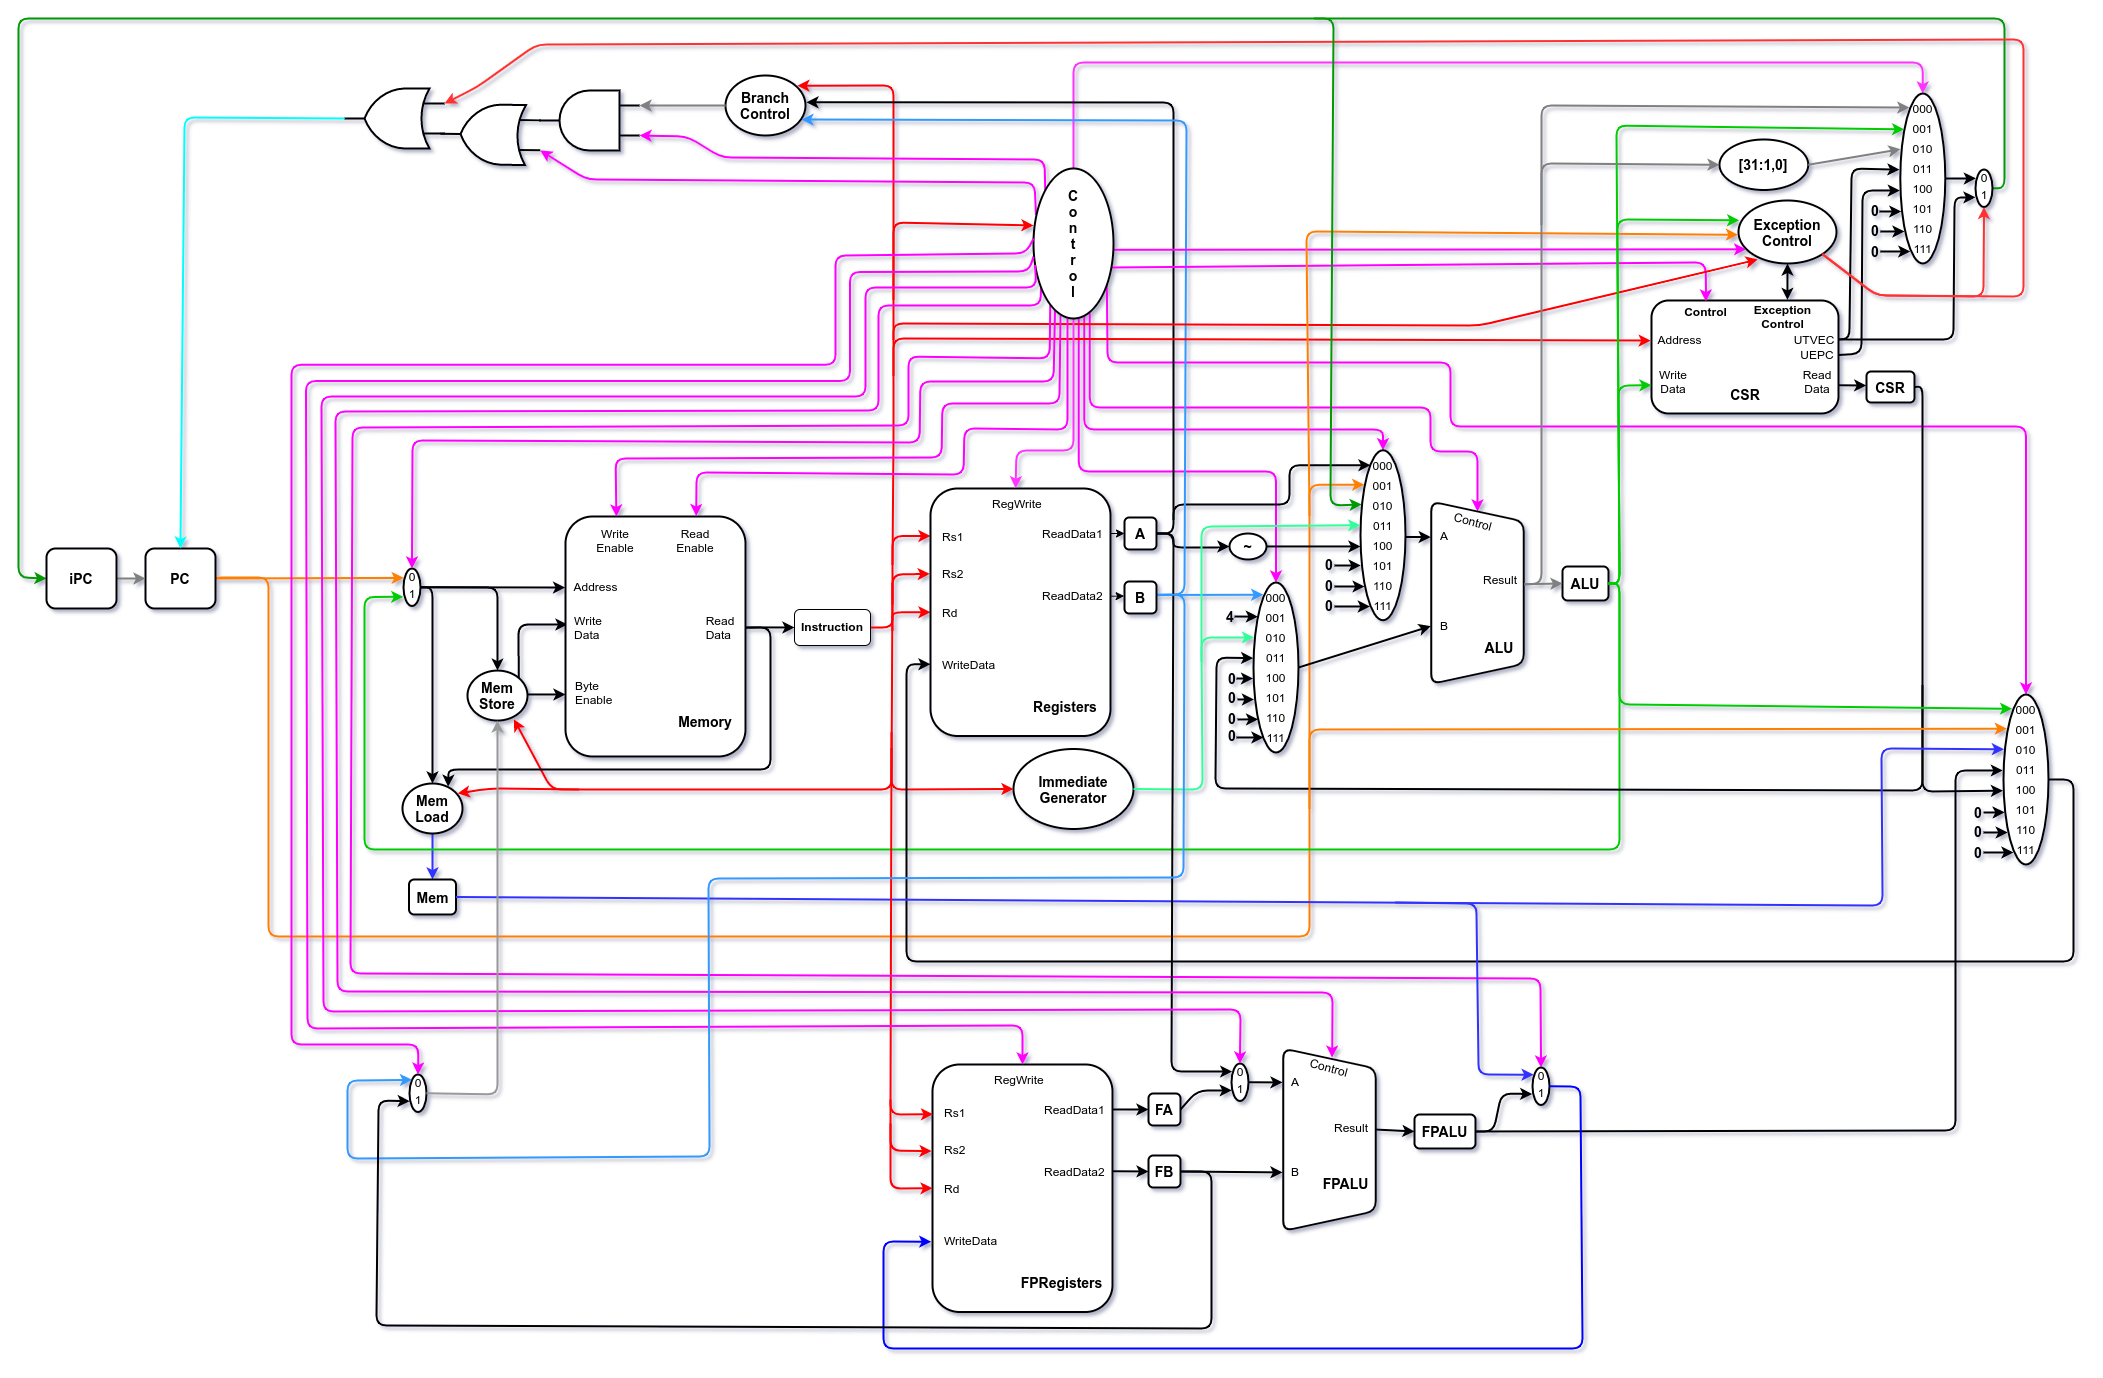
\includegraphics[width=.9\linewidth]{../images/uarch_diagrams/multicycle-RV32IMF.png}
            \caption{Diagrama da implementação da \textit{ISA} RV32IMF na
            microarquitetura multiciclo}\label{fig:diagram_rv32imf_multi}
        \end{figure}


    \subsection{Microarquitetura \textit{Pipeline} de 5 Estágios (Incompleto)}
        { Os processadores \textit{pipeline} com extensões I e IM são
            implementados conforme o diagrama da Figura~\ref{fig:diagram_rv32i_pipe}.
            Seus cinco estágios são:
            \begin{enumerate}
                \item \textit{Instruction Fetch}
                \item \textit{Instruction Decode}
                \item \textit{Execution}
                \item \textit{Memory Stage}
                \item \textit{Write Back}
            \end{enumerate}
        }
        { A frequência máxima do seu \textit{clock} é limitada pela operação
            mais lenta da unidade lógica e aritmética na terceira etapa do
            \textit{pipeline}.
        }

        \begin{figure}[H]
        \centering
            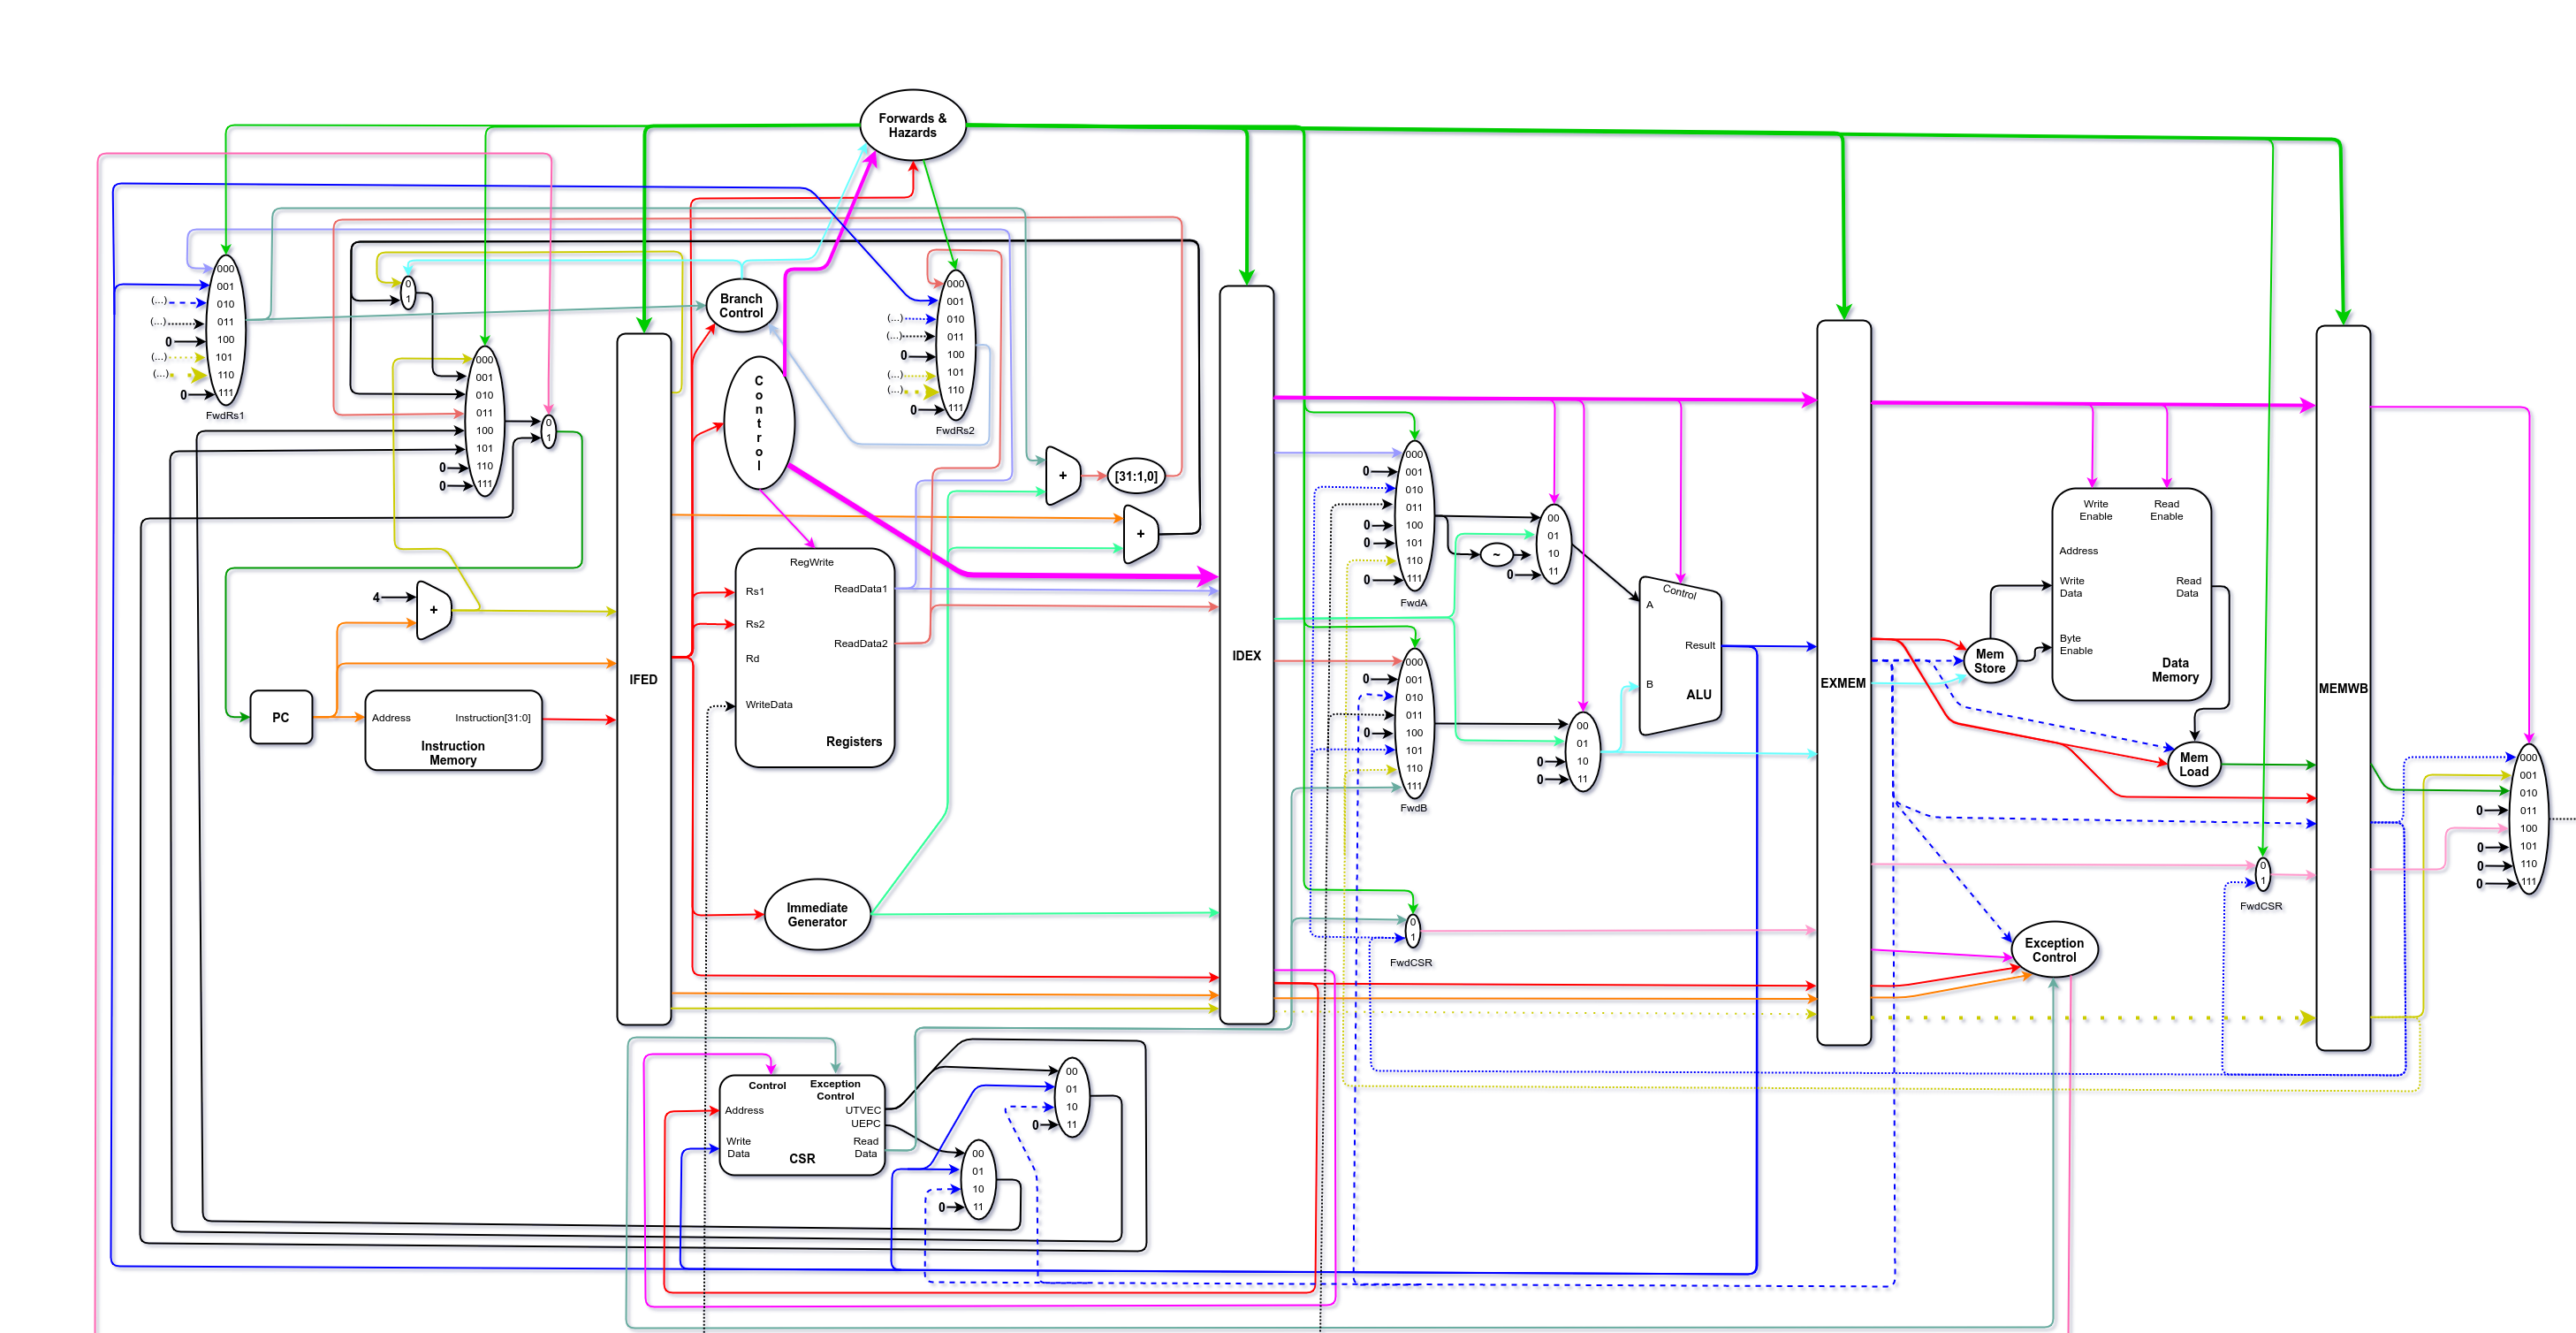
\includegraphics[width=.9\linewidth]{../images/uarch_diagrams/pipeline-RV32I-RV32IM.png}
            \caption{Diagrama da implementação das \textit{ISAs} RV32I e RV32IM na
            microarquitetura \textit{pipeline} de 5 estágios}\label{fig:diagram_rv32i_pipe}
        \end{figure}

        { O processador \textit{pipeline} com extensões IMF é implementado conforme
            o diagrama da Figura~\ref{fig:diagram_rv32imf_pipe}.
        }

        \begin{figure}[H]
        \centering
            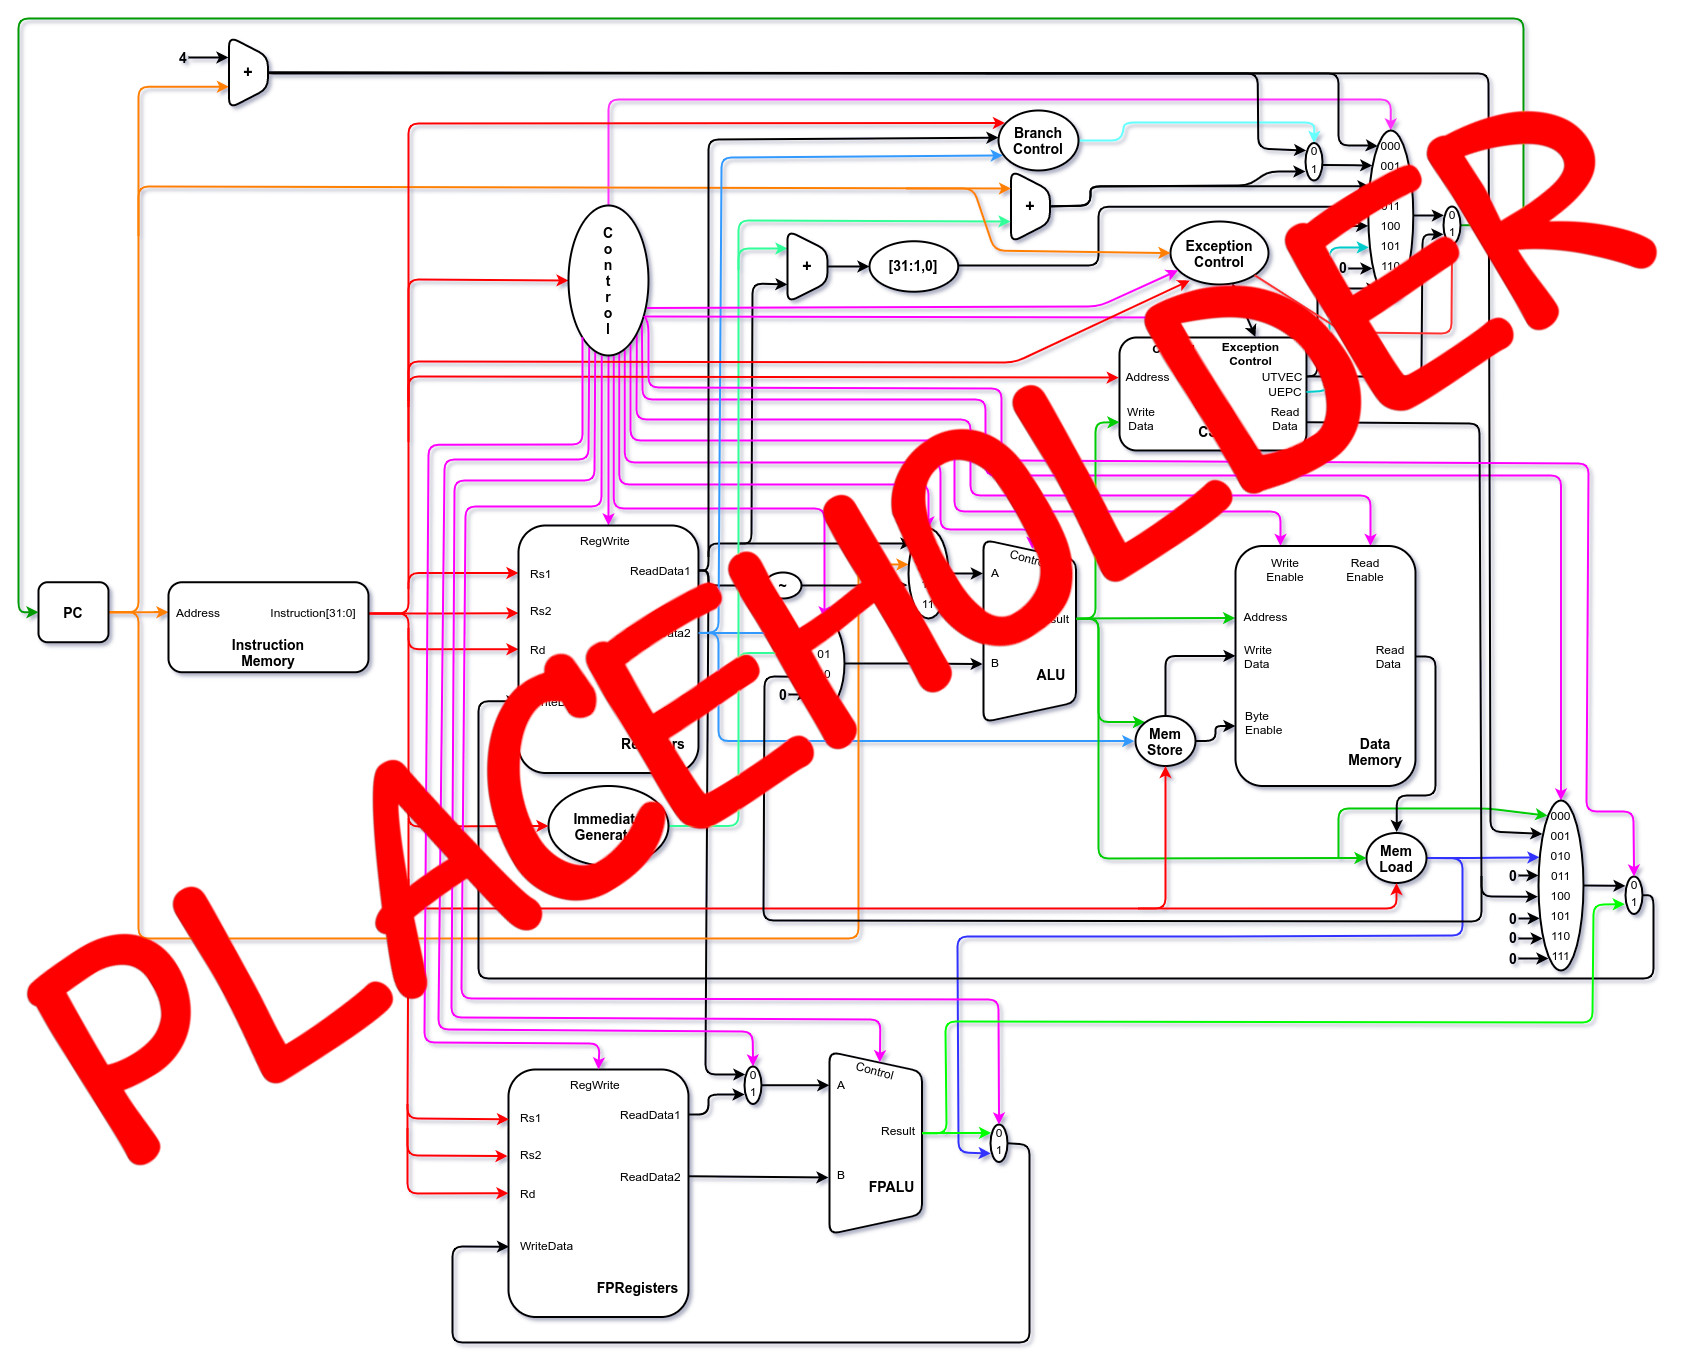
\includegraphics[width=.9\linewidth]{../images/uarch_diagrams/pipeline-RV32IMF.png}
            \caption{Diagrama da implementação da \textit{ISA} RV32IMF na
            microarquitetura \textit{pipeline} de 5 estágios}\label{fig:diagram_rv32imf_pipe}
        \end{figure}


\clearpage
\section{Chamadas de sistema}
    { A pasta \texttt{system} contém a implementação das chamadas de sistema do
        processador. O código \textit{assembly} deve incluir o arquivo
        \texttt{system/MACROS.s} no início do programa e o arquivo
        \texttt{system/SYSTEM.s} ao final do programa.
    }
    \begin{lstlisting}
# Inicio do programa
.include "MACROS.s"

# Dados do programa
.data
    ...

# Instrucoes do programa
.text
    ...

# Chamadas de sistema
.include "SYSTEM.s"
    \end{lstlisting}

    { O arquivo \texttt{MACROS.s} insere macros que testam se o programa
        está sendo executado no \texttt{Rars}, na \texttt{FPGA} ou no
        \texttt{ModelSim} para decidir o uso de determinadas \textit{syscalls},
        e também fornece a implementação por \textit{software} de algumas
        instruções caso a extensão necessária não esteja implementada no processador,
        como instruções de multiplicação. Os endereços de memória dos periféricos
        acessados por \textit{MMIO} também estão presentes como definições
        \texttt{.eqv} para facilitar a implementação dos programas.
    }

    { Já o arquivo \texttt{SYSTEM.s} implementa o \textit{kernel} do sistema,
        tratando exceções e executando as \textit{syscalls}. As chamadas de
        sistema implementadas são apresentadas na Tabela~\ref{table:syscalls}.
    }

    { Como o processador implementado não possui memória reservada para o
        \textit{kernel}, sua posição inicial de memória começa imediatamente
        após a última instrução do programa implementado, e por isso deve ser
        incluído no final do arquivo. O arquivo de macros deve ser adicionado
        no início do programa, pois ele é responsável por gravar o endereço inicial
        do nível privilegiado no \textit{CSR UTVEC} e ativar as interrupções.
    }

    \begin{longtable}{|l|c|p{3cm}|l |}
        \caption{Tabela de \textit{syscalls} implementadas.}\label{table:syscalls}\\
        \hline
        \textit{syscall}                    & \texttt{a7}             & Argumentos                & Operação\\*
        \hline
        \endfirsthead
        \hline
        \textit{syscall}                    & \texttt{a7}             & Argumentos                & Operação\\*
        \hline
        \endhead
        \multirow{5}{*}{Print Integer}      & \multirow{5}{*}{\parbox{0.6cm}{\centering 1 ou 101}}
              & \texttt{a0 =} inteiro     & \multirow{5}{*}{\parbox{7cm}{Imprime no \textit{frame} \texttt{a4} o número inteiro \texttt{a0} (complemento de 2) na
                                                posição \texttt{(a1,a2)} com as cores \texttt{a3[7:0]} de \textit{foreground} e \texttt{a3[15:8]} de \textit{background}.}}\\*
            & & \texttt{a1 =} coluna      & \\*
            & & \texttt{a2 =} linha       & \\*
            & & \texttt{a3 =} cores       & \\*
            & & \texttt{a4 =} frame       & \\
        \hline
        \multirow{5}{*}{Print Float}        & \multirow{5}{*}{\parbox{0.6cm}{\centering 2 ou 102}}
              & \texttt{fa0 =} float      & \multirow{5}{*}{\parbox{7cm}{Imprime no \textit{frame} \texttt{a4} o número de ponto flutuante \texttt{fa0} na
                                                posição \texttt{(a1,a2)} com as cores \texttt{a3[7:0]} de \textit{foreground} e \texttt{a3[15:8]} de \textit{background}.}}\\*
            & & \texttt{a1 =} coluna      & \\*
            & & \texttt{a2 =} linha       & \\*
            & & \texttt{a3 =} cores       & \\*
            & & \texttt{a4 =} frame       & \\
        \hline
        \multirow{5}{*}{Print String}       & \multirow{5}{*}{\parbox{0.6cm}{\centering 4 ou 104}}
              & \texttt{a0 =} endereço da string  & \multirow{5}{*}{\parbox{7cm}{Imprime no \textit{frame} \texttt{a4} a \textit{string} iniciada no endereço \texttt{a0} e terminada
                                                        em \textit{NULL} na posição \texttt{(a1,a2)} com as cores \texttt{a3[7:0]} de \textit{foreground} e \texttt{a3[15:8]} de \textit{background}.}}\\*
            & & \texttt{a1 =} coluna      & \\*
            & & \texttt{a2 =} linha       & \\*
            & & \texttt{a3 =} cores       & \\*
            & & \texttt{a4 =} frame       & \\
        \hline
        \multirow{3}{*}{Read Int}           & \multirow{3}{*}{\parbox{0.6cm}{\centering 5 ou 105}}
            &                               & \multirow{3}{*}{\parbox{7cm}{Retorna em \texttt{a0} o valor do inteiro em complemento de 2 lido do teclado.}}\\*
            & & & \\*
            & & & \\
        \hline
        \multirow{3}{*}{Read Float}         & \multirow{3}{*}{\parbox{0.6cm}{\centering 6 ou 106}}
            &                               & \multirow{3}{*}{\parbox{7cm}{Retorna em \texttt{a0} o valor do \textit{float} com precisão simples lido do teclado.}}\\*
            & & & \\*
            & & & \\
        \hline
        \multirow{3}{*}{Read String}        & \multirow{3}{*}{\parbox{0.6cm}{\centering 8 ou 108}}
            & \texttt{a0 =} endereço do buffer    & \multirow{3}{*}{\parbox{7cm}{Escreve no \textit{buffer} iniciado em \texttt{a0} os caracteres lidos, terminando com um caracter \textit{NULL}.}}\\*
            & & \texttt{a1 =} número máximo de caracteres & \\*
            & & & \\
        \hline
        \multirow{3}{*}{Exit}               & \multirow{3}{*}{\parbox{0.6cm}{\centering 10 ou 110}}
            &                               & \multirow{3}{*}{\parbox{7cm}{Retorna ao sistema operacional. Na \textit{DE1-SoC}, trava o processador.}}\\*
            & & & \\*
            & & & \\
        \hline
        \multirow{5}{*}{Print Char}         & \multirow{5}{*}{\parbox{0.6cm}{\centering 11 ou 111}}
              & \texttt{a0 =} char ASCII  & \multirow{5}{*}{\parbox{7cm}{Imprime no \textit{frame} \texttt{a4} o caracter \texttt{a0} na
                                                posição \texttt{(a1,a2)} com as cores \texttt{a3[7:0]} de \textit{foreground} e \texttt{a3[15:8]} de \textit{background}.}}\\*
            & & \texttt{a1 =} coluna      & \\*
            & & \texttt{a2 =} linha       & \\*
            & & \texttt{a3 =} cores       & \\*
            & & \texttt{a4 =} frame       & \\
        \hline
        \multirow{3}{*}{Read Char}          & \multirow{3}{*}{\parbox{0.6cm}{\centering 12 ou 112}}
            &                               & \multirow{3}{*}{\parbox{7cm}{Retorna em \texttt{a0} o valor ASCII do caracter lido do teclado.}}\\*
            & & & \\*
            & & & \\
        \hline
        \multirow{3}{*}{Time}               & \multirow{3}{*}{\parbox{0.6cm}{\centering 30 ou 130}}
            &                               & \multirow{3}{*}{\parbox{7cm}{Retorna o tempo do sistema em \textit{ms}, com os 32 \textit{bits} menos significativos em \texttt{a0}
                                                e os 32 \textit{bits} mais significativos em \texttt{a1}.}}\\*
            & & & \\*
            & & & \\
        \hline
        \multirow{4}{*}{MIDI Out Assíncrono }   & \multirow{4}{*}{\parbox{0.6cm}{\centering 31 ou 131}}
              & \texttt{a0 =} pitch       & \multirow{4}{*}{\parbox{7cm}{Gera o som definido e retorna imediatamente.}}\\*
            & & \texttt{a1 =} duração (\textit{ms}) & \\*
            & & \texttt{a2 =} instrumento & \\*
            & & \texttt{a3 =} volume      & \\
        \hline
        \multirow{3}{*}{Sleep}              & \multirow{3}{*}{\parbox{0.6cm}{\centering 32 ou 132}}
            & \texttt{a0 =} duração (\textit{ms}) & \multirow{3}{*}{\parbox{7cm}{Coloca o processador em \textit{sleep} por \texttt{a1} \textit{ms}.}}\\*
            & & & \\*
            & & & \\
        \hline
        \multirow{4}{*}{MIDI Out Síncrono }     & \multirow{4}{*}{\parbox{0.6cm}{\centering 33 ou 133}}
              & \texttt{a0 =} pitch       & \multirow{4}{*}{\parbox{7cm}{Gera o som definido e retorna após o término da execução da nota.}}\\*
            & & \texttt{a1 =} duração (\textit{ms}) & \\*
            & & \texttt{a2 =} instrumento & \\*
            & & \texttt{a3 =} volume      & \\
        \hline
        \multirow{5}{*}{Print Integer}      & \multirow{5}{*}{\parbox{0.6cm}{\centering 34 ou 134}}
              & \texttt{a0 =} inteiro     & \multirow{5}{*}{\parbox{7cm}{Imprime no \textit{frame} \texttt{a4} o número inteiro \texttt{a0} em formato hexadecimal na
                                                posição \texttt{(a1,a2)} com as cores \texttt{a3[7:0]} de \textit{foreground} e \texttt{a3[15:8]} de \textit{background}.}}\\*
            & & \texttt{a1 =} coluna      & \\*
            & & \texttt{a2 =} linha       & \\*
            & & \texttt{a3 =} cores       & \\*
            & & \texttt{a4 =} frame       & \\
        \hline
        \multirow{5}{*}{Print Integer Unsigned} & \multirow{5}{*}{\parbox{0.6cm}{\centering 36 ou 136}}
              & \texttt{a0 =} inteiro     & \multirow{5}{*}{\parbox{7cm}{Imprime no \textit{frame} \texttt{a4} o número inteiro \texttt{a0} sem sinal na
                                                posição \texttt{(a1,a2)} com as cores \texttt{a3[7:0]} de \textit{foreground} e \texttt{a3[15:8]} de \textit{background}.}}\\*
            & & \texttt{a1 =} coluna      & \\*
            & & \texttt{a2 =} linha       & \\*
            & & \texttt{a3 =} cores       & \\*
            & & \texttt{a4 =} frame       & \\
        \hline
        \multirow{3}{*}{Rand}               & \multirow{3}{*}{\parbox{0.6cm}{\centering 41 ou 141}}
            & & \multirow{3}{*}{\parbox{7cm}{Retorna um número pseudorandômico de 32 \textit{bits} em \texttt{a0}.}}\\*
            & & & \\*
            & & & \\
        \hline
        \multirow{6}{*}{Draw Line}          & \multirow{6}{*}{\parbox{0.6cm}{\centering 47 ou 147}}
              & \texttt{a0 =} $x_0$       & \multirow{6}{*}{\parbox{7cm}{Desenha no \textit{frame} \texttt{a5} uma linha reta do ponto \texttt{(a0,a1)} até o ponto \texttt{(a2,a3)}
                                                com as cores \texttt{a3[7:0]} de \textit{foreground} e \texttt{a3[15:8]} de \textit{background}.}}\\*
            & & \texttt{a1 =} $y_0$       & \\*
            & & \texttt{a2 =} $x_1$       & \\*
            & & \texttt{a3 =} $y_1$       & \\*
            & & \texttt{a4 =} cor         & \\*
            & & \texttt{a5 =} frame       & \\
        \hline
        \multirow{3}{*}{Read Char}          & \multirow{3}{*}{\parbox{0.6cm}{\centering 48 ou 148}}
            & \texttt{a0 =} cor           & \multirow{3}{*}{\parbox{7cm}{Preenche o \textit{frame} \texttt{a1} com a cor \texttt{a0}.}}\\*
            & & \texttt{a1 =} frame       & \\*
            & & & \\
        \hline
    \end{longtable}

    { As \textit{ecalls} \texttt{1XX} são utilizadas no \textit{Rars} pelas
        ferramentas \textit{Bitmap Display Tool} e \textit{Keyboard Display MMIO
        Tool}, que foram customizadas para funcionar de maneira idêntica quando
        o programa é executado na \textit{FPGA}.
    }


    \section{Utilizando o RARS}
    { Brevemente apresentado na Seção~\ref{rars_cap2}, a \textit{IDE RARS} é uma
        ferramenta essencial da \textit{toolchain} desse trabalho. Presente na
        pasta \texttt{tools/rars}, há duas versões customizadas do programa.
        As customizações permitem simular a saída de vídeo (exceto o menu \textit{OSD})
        e entrada do teclado da mesma forma que na \textit{FPGA}.
    }

    { Além da sua interface de edição de texto mostrada na Figura~\ref{fig:rars},
        há também a visualização do simulador. Nela é mostrado o código montado,
        os bancos de registradores e outras ferramentas como o simulador de
        \textit{display}, como visto na Figura~\ref{fig:rars_debug}. É possível
        executar o código instrução por instrução, fazer o ``\textit{rewind}''
        da execução e definir \textit{breakpoints}. Suas funções de \textit{debug}
        são importantes tanto para validar o código produzido quando para executar
        passo-a-passo junto com a \textit{FPGA} para identificar discrepâncias
        na implementação do \textit{hardware}.
    }

    \begin{figure}[H]
    \centering
        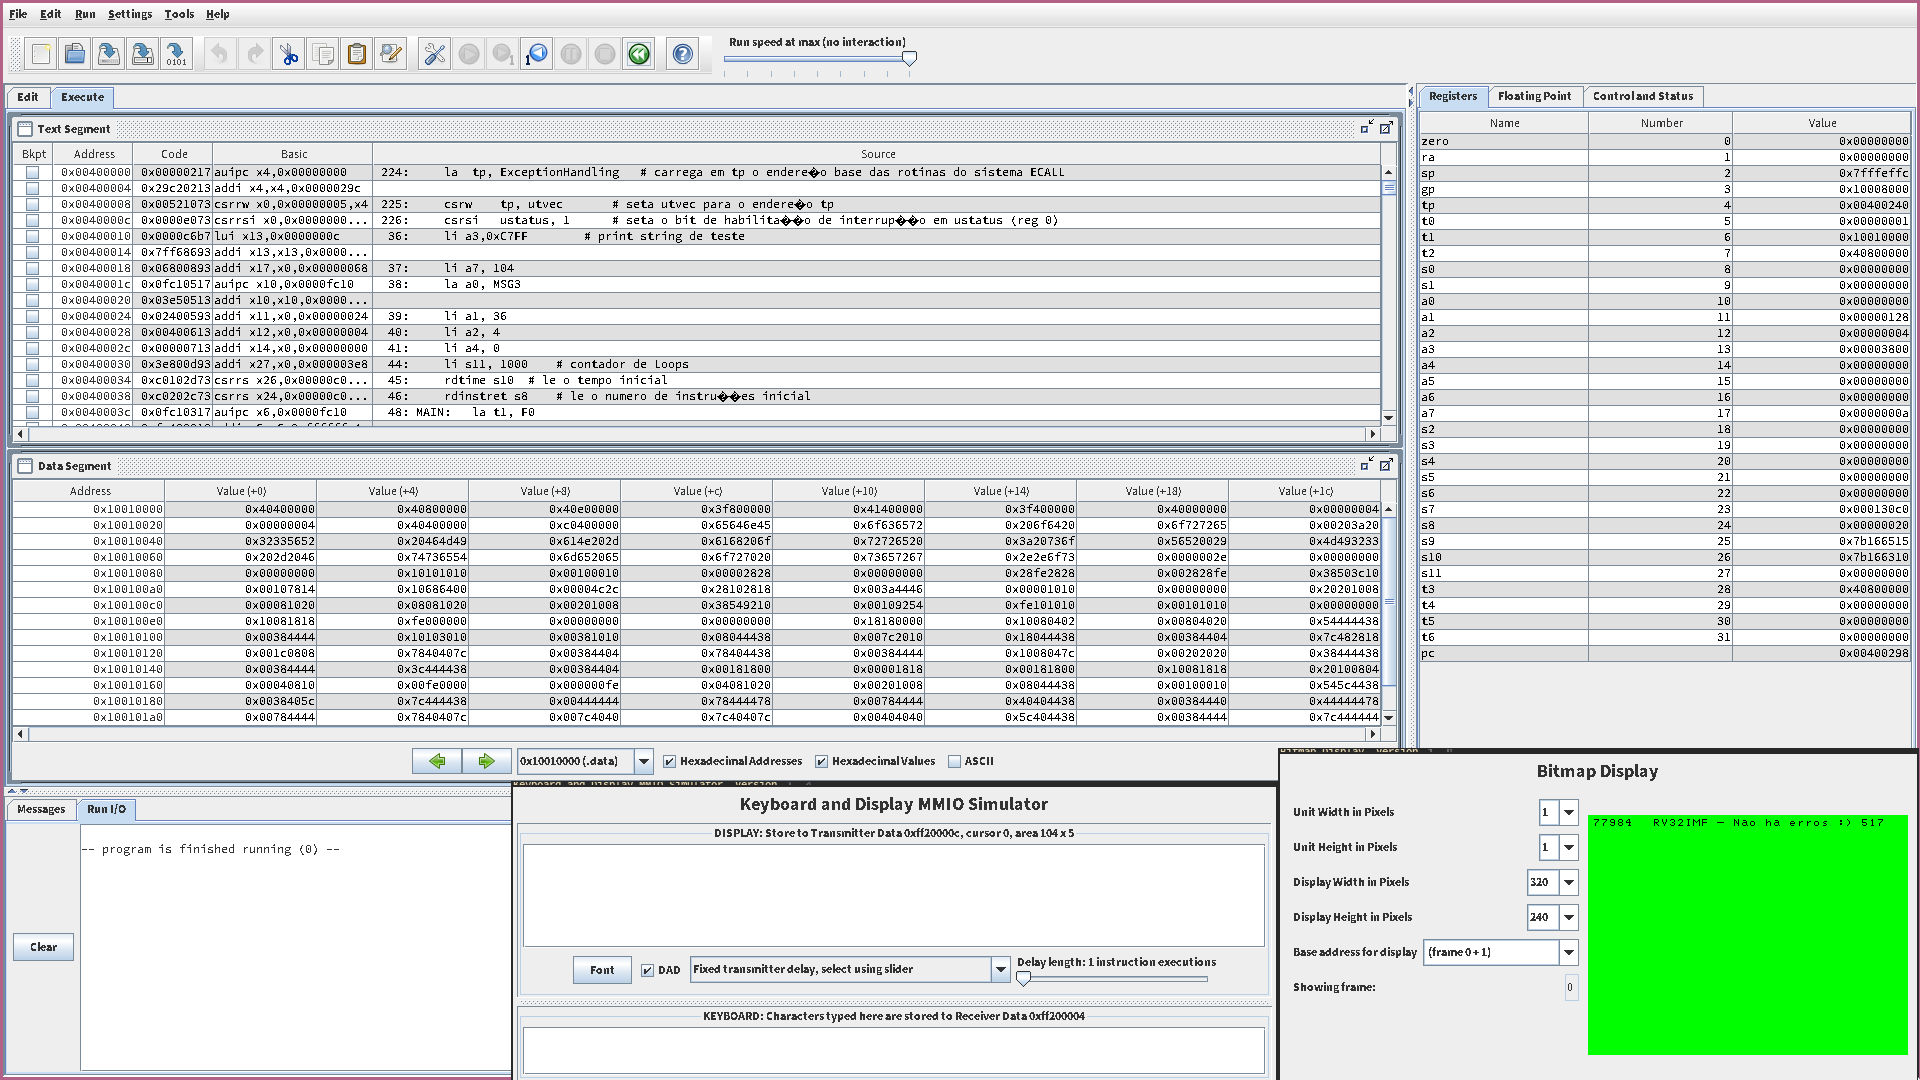
\includegraphics[width=.9\linewidth]{../images/rars_debug.png}
        \caption{Exibição do \textit{frame} de vídeo da \textit{FPGA}}
        \label{fig:rars_debug}
    \end{figure}

    { O \textit{RARS} também é usado para gerar os arquivos \texttt{.mif} para
        inicializar a memória da \textit{FPGA} clicando no menu \texttt{File > Dump Memory}
        ou usando o atalho de teclado \texttt{Ctrl+d}. São gerados dois arquivos,
        um contendo a memória de dados e o outro a memória de texto.
    }

    { Os arquivos \texttt{core/default\_data.mif} e \texttt{core/default\_text.mif}
        são os arquivos gravados na memória da \textit{FPGA} quando é realizada a
        síntese do processador. Esses arquivos também podem ser alterados a tempo
        de execução usando a ferramenta \texttt{Tools > In-System Memory Content
        Editor} do \textit{Quartus}. A pasta \texttt{test/assembly\_testbenches}
        possui alguns programas em \textit{assembly} para testar a \textit{FPGA}.
        Já na pasta \texttt{test/mif\_library}, existem testes já montados prontos
        para gravação na placa de desenvolvimento.
    }

    \section{Interface de vídeo e depuração}
    { A interface de vídeo possui resolução de 320x240 \textit{pixels} com 8
        \textit{bits} de cor para cada pixel. Efetivamente, a interface de vídeo
        possui 255 cores diferentes e uma cor utilizada como transparência, o
        magenta \texttt{0xC7}. Ela também conta com dois \textit{framebuffers},
        permitindo renderizar duas imagens diferentes e alternar entre elas, ou
        se aplicado em um jogo, permite a transição de \textit{frames} sem
        \textit{flickering}: enquanto um \textit{frame} é exibido, o outro
        \textit{framebuffer} é construído com as imagens do próximo \textit{frame},
        e quando pronto, a tela é atualizada com o novo \textit{frame}
        completamente renderizado.
    }

    { A conexão do vídeo do sistema é feita por interface VGA, podendo se
        conectar a qualquer monitor com entrada VGA. A resolução real da
        interface é de 640x480 \textit{pixels} com taxa de atualização de 59 Hz
        por questões de compatibilidade com os monitores. Cada \textit{pixel}
        da interface de vídeo representa uma célula de 4 \textit{pixels} na
        saída de vídeo real. A saída de vídeo VGA também possui 24 \textit{bits}
        de cor, pois o controlador faz a conversão das cores em 8 \textit{bits}
        para três canais de 8 \textit{bits}, um verde, um vermelho e um azul.
    }
    \begin{figure}[H]
    \centering
        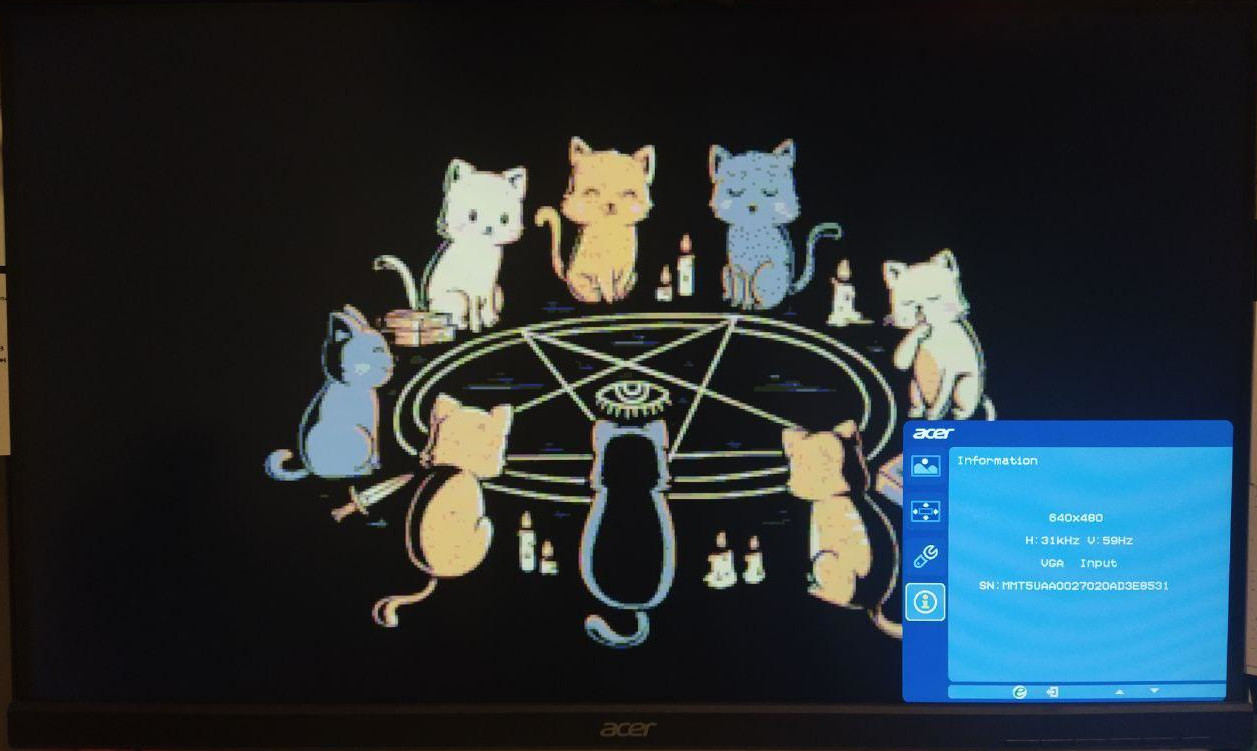
\includegraphics[width=.9\linewidth]{../images/osd/display.jpg}
        \caption{Exibição do \textit{frame} de vídeo da \textit{FPGA}}
        \label{fig:display_cats}
    \end{figure}

    { Acionando um \textit{switch} da \textit{FPGA}, é mostrado por cima do
        \textit{frame} um \textit{menu On Screen Display} que mostra o valor
        atual contido nos bancos de registradores do processador, incluindo os
        \textit{CSRs} e, caso a extensão F esteja implementada, outro
        \textit{switch} permite alternar entre a visualização dos registradores
        de ponto flutuante e os de ponto fixo.
    }
    \begin{figure}[H]
    \centering
        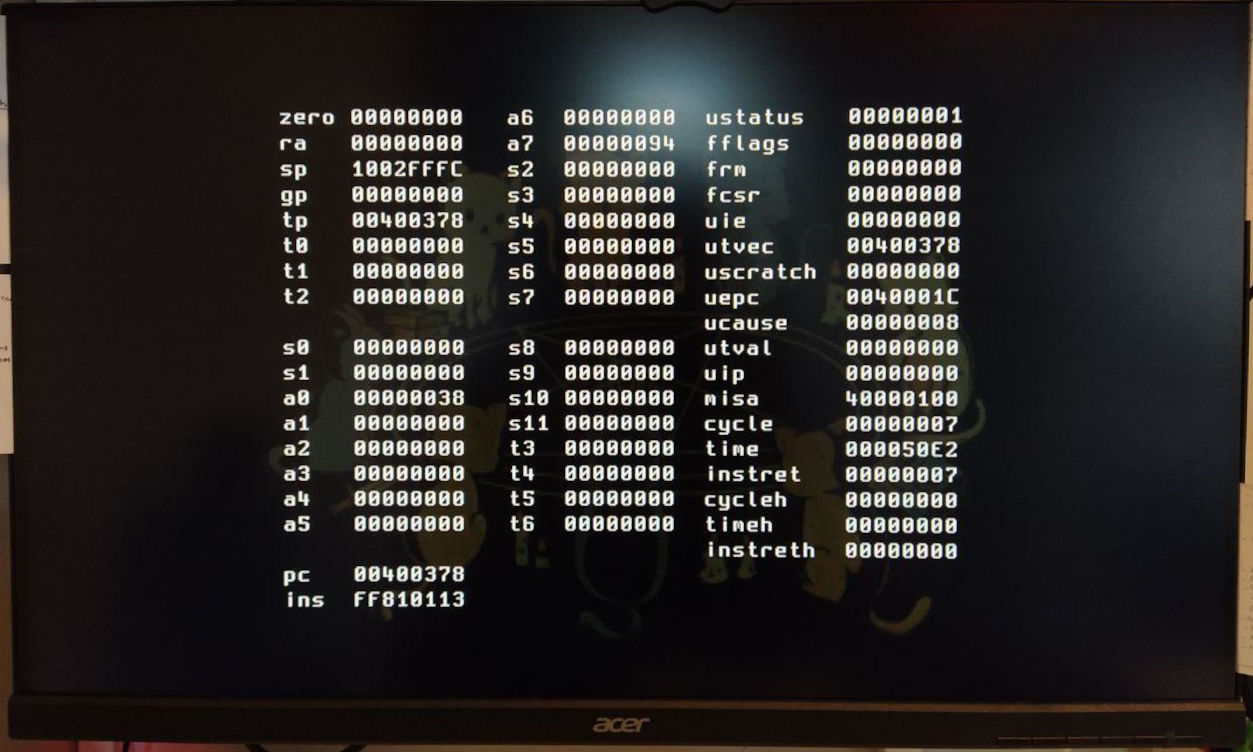
\includegraphics[width=.9\linewidth]{../images/osd/display_osd.jpg}
        \caption{\textit{Menu OSD} exibindo os valores dos registradores do processador}
        \label{fig:display_cats_osd}
    \end{figure}

    { O \textit{menu OSD} é implementado como uma matriz de 52x24 caracteres
        monoespaçados. Na matriz, os caracteres que não mudam com o tempo, como
        é o caso do nome dos registradores, são representados por um parâmetro
        correspondente ao próprio caracter. Já os valores que se alteram, como
        o valor dos registradores, são representados por um parâmetro
        \textit{placeholder}, e o valor a ser mostrado na tela é obtido usando
        uma tabela de \textit{lookup}. O projeto do \textit{menu OSD} foi pensado
        de forma que possa ser modificado para expansão ou utilização em outras
        arquiteturas de processadores de maneira simples.
    }

\clearpage
\section{Configuração e síntese do processador pelo Quartus}
    { O \textit{software} utilizado para a síntese do processador, fornecimento
        de \textit{IPs} como as de memória e operações de ponto flutuante,
        gravação do \textit{soft-core}, dentre outras funcionalidades é o
        \textit{Intel Quartus Lite v18.1}. Versões superiores são compatíveis com
        menos sistemas operacionais e/ou não possuem todos os \textit{IPs}
        necessários para a síntese do processador.
    }
    \begin{figure}[H]
    \centering
        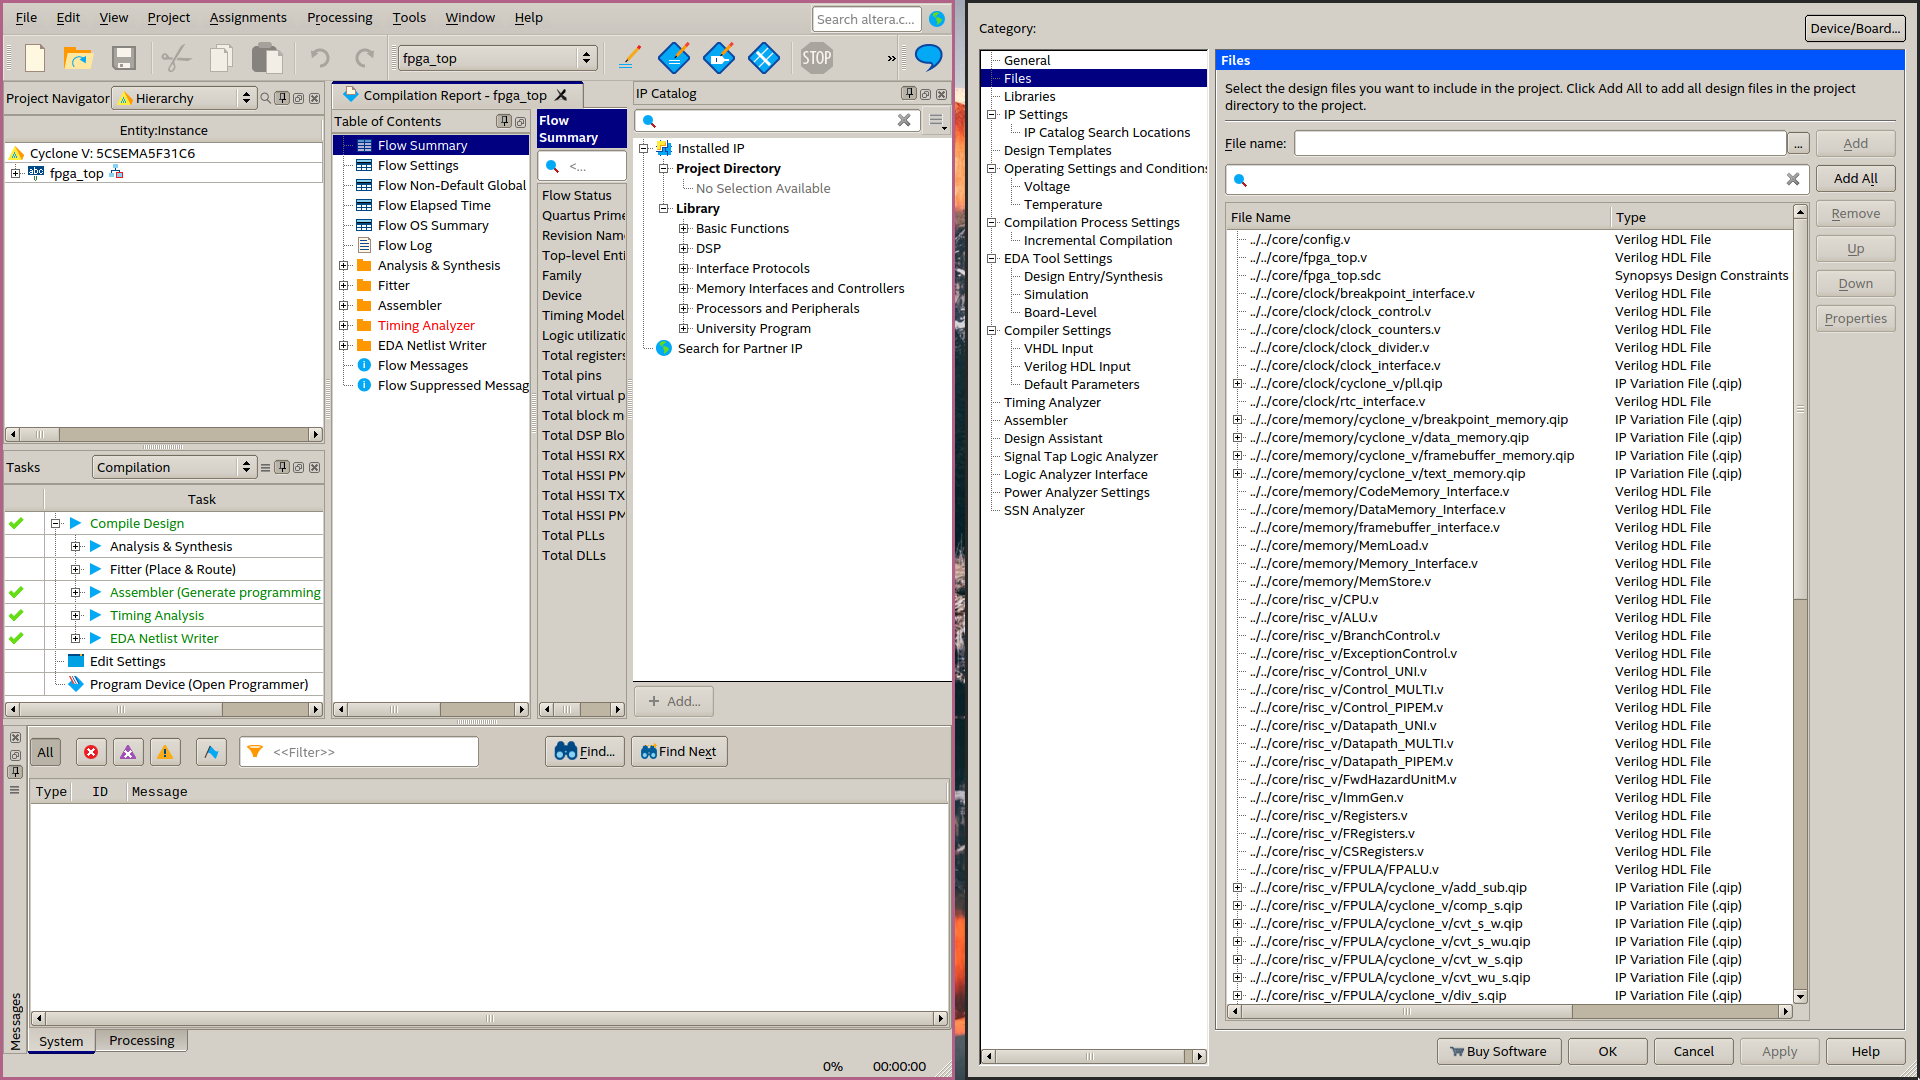
\includegraphics[width=.9\linewidth]{../images/quartus/files_config.png}
        \caption{\textit{Intel Quartus Lite v18.1} com a janela de configurações
            do projeto}\label{fig:quartus_files_config}
    \end{figure}

    { Todas as configurações do projeto também podem ser alteradas manualmente
        no arquivo \texttt{project/de1\_soc/fpga\_top.qsf}. Para ativar ou desativar
        os pinos do \textit{chip} da \textit{FPGA} que conectam os periféricos
        da placa, é preferível que a edição seja feita diretamente no arquivo
        de configuração, comentando ou descomentando a declaração dos pinos.
    }

    { Para realizar a síntese completa do processador para utilizá-lo na \textit{FPGA},
        basta acessar o menu \texttt{Processing > Start Compilation} ou utilizar
        o atalho \texttt{Ctrl + L} ou clicar no ícone de \textit{"Play"}
        na barra de tarefas do programa. Assim, as etapas de Análise e Síntese,
        \textit{Placing} e \textit{Routing}, \textit{Assembler} e
        \textit{Timing Analysis} serão realizadas, e, caso não ocorram erros
        durante o processo, o \textit{soft-core} estará pronto para ser
        gravado na \textit{FPGA} utilizando o arquivo \textit{.mif} gerado.
    }


\section{Simulação do processador pelo Quartus e ModelSim}
    { O projeto possui um \textit{testbench} em \textit{Verilog} para simular as
        entradas e saídas da \textit{FPGA} que o usuário operaria, como os botões
        e \textit{switches}. Ele configura a rotina de reinicialização da placa
        após o \textit{power-up} e define por quanto tempo a simulação será
        executada.
    }

    { O \textit{script} \texttt{test/simulation\_scripts/de1\_soc\_rtl.do} é
        necessário para realizar a simulação de forma correta. O \textit{script}
        gerado automaticamente pelo \textit{Quartus} apresenta problemas que
        impedem que a simulação seja executada corretamente, além de não gerar
        o arquivo de saída da simulação no formato desejado.
    }
    \begin{figure}[H]
    \centering
        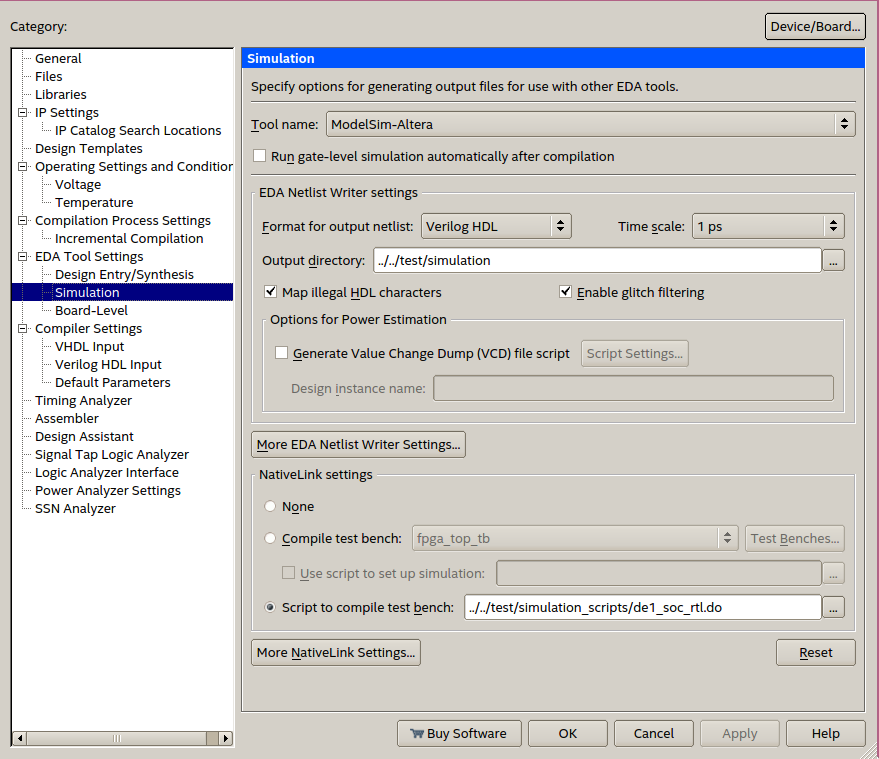
\includegraphics[width=.6\linewidth]{../images/quartus/simulation_config.png}
        \caption{Janela de configuração da simulação no \textit{Quartus}.}
        \label{fig:quartus_simulation_config}
    \end{figure}

    { Por limitações do \textit{Quartus}, não é possível simular
        \textit{FPGAs Cyclone V} a nível de portas lógicas, somente sendo possível
        fazer a simulação \textit{RTL}. Por outras limitações no programa, o
        \textit{script .do} produzido manualmente só é executado usando o
        \textit{menu} \texttt{Tools > Run Simulation Tool > Gate Level Simulation},
        que, apesar do nome, executará uma simulação \textit{RTL}. A opção
        \texttt{Tools > Run Simulation Tool > RTL Simulation} utiliza o \textit{script}
        .do gerado automaticamente, e falha ao ser processado.
    }

    \begin{figure}[H]
    \centering
        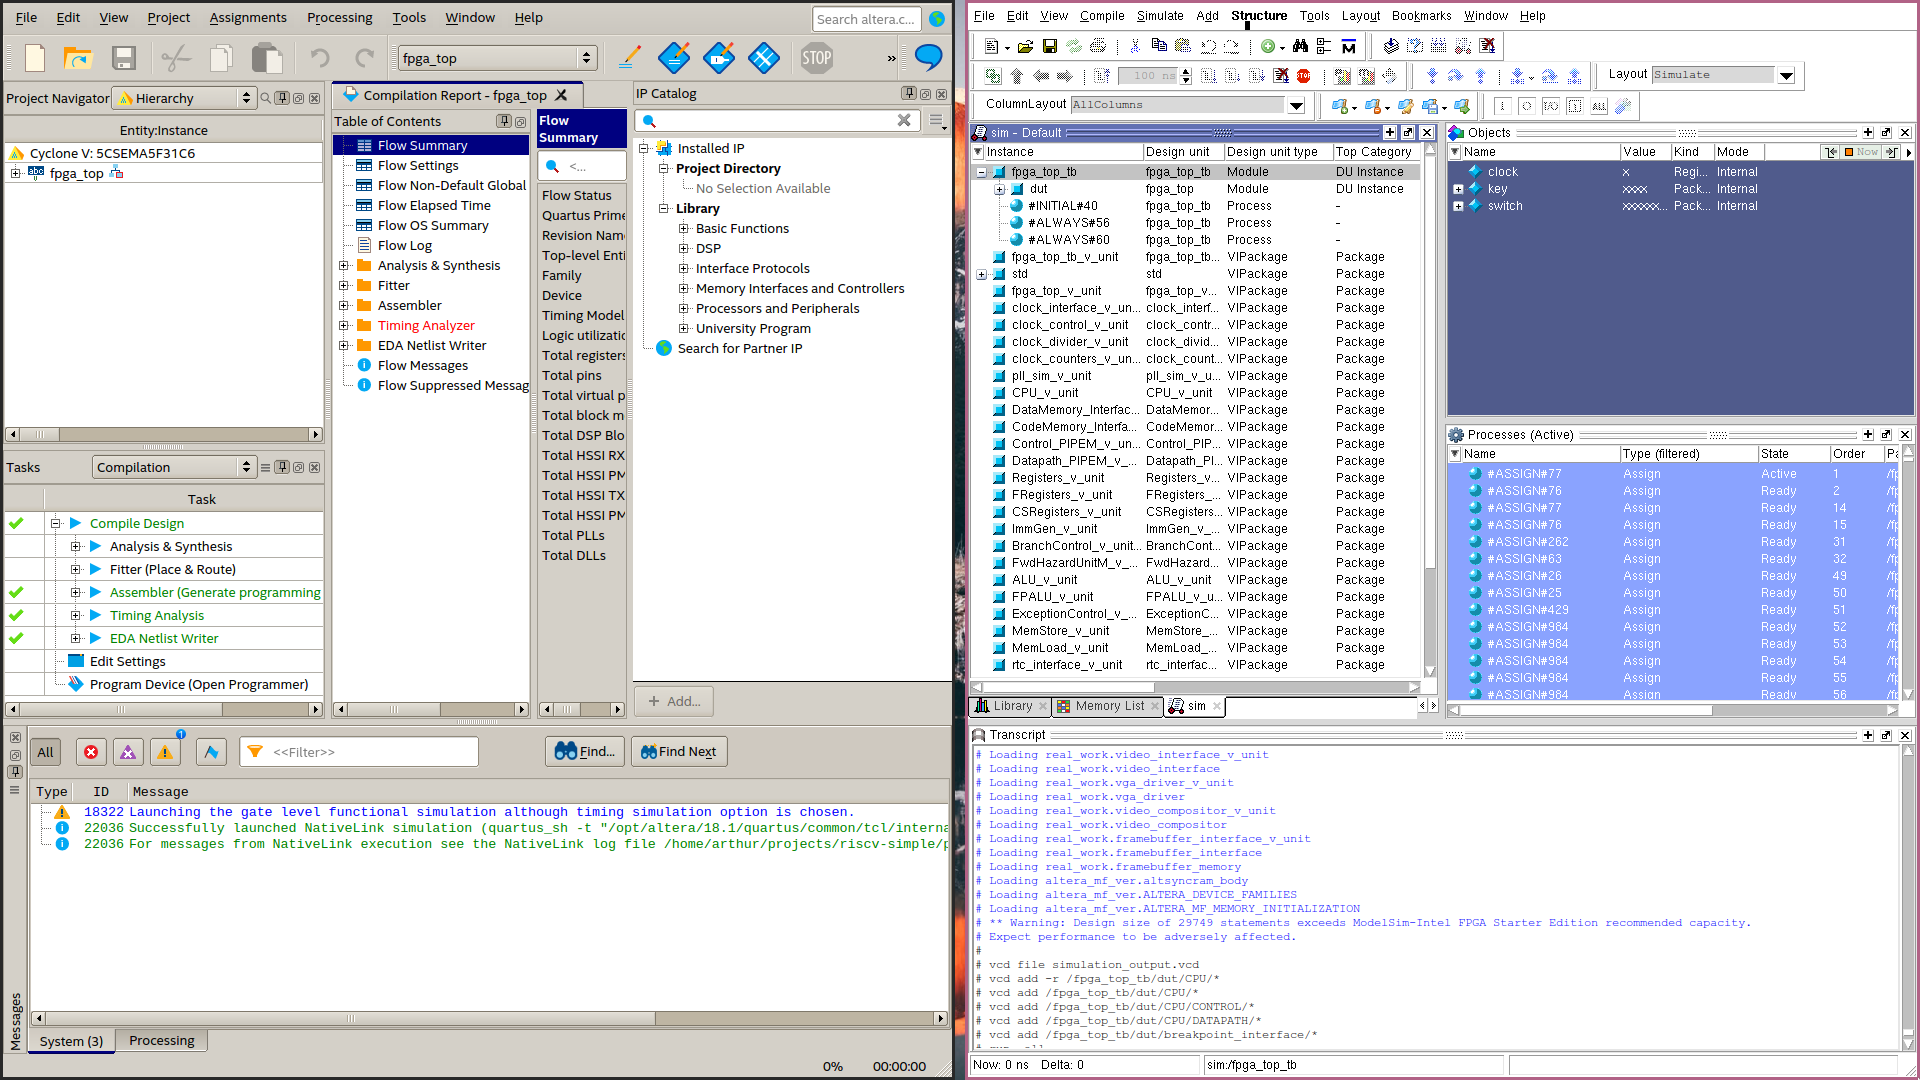
\includegraphics[width=.75\linewidth]{../images/quartus/quartus_modelsim.png}
        \caption{O \textit{script NativeLink} invoca o \textit{ModelSim} passando
            o \textit{script .do} com as informações de como simular o sistema}
        \label{fig:quartus_modelsim}
    \end{figure}

    { Ao executar a simulação, os \textit{scripts NativeLink} iniciarão o
        programa \textit{ModelSim}, carregando o \textit{script .do} customizado,
        conforme mostrado na Figura~\ref{fig:quartus_modelsim}. Ao finalizar a
        simulação, um arquivo \texttt{.vcd} será gerado e poderá ser analisado
        em \textit{softwares} de visualização de formatos de onda, como o
        \textit{GTKWave} ou o próprio \textit{ModelSim}.
    }

    { Ao carregar um arquivo \texttt{.vcd} no \textit{GTKWave}, a hierarquia
        dos módulos é mostrada em uma árvore no canto superior esquerdo da tela.
        Ao clicar no nó desejado da árvore, os sinais do módulo serão mostrados
        no canto inferior esquerdo da tela. Para visualizá-lo, basta clicar e
        arrastar o sinal para a área \textit{Signals}. A Figura~\ref{fig:gtkwave_generic}
        mostra uma visualização dos sinais escolhidos. Na pasta \texttt{test/gtkwave}
        do projeto, existe um arquivo \texttt{.gtkw} para cada uma das nove
        configurações do \textit{soft-core} com sinais predefinidos.
    }

    \begin{figure}[H]
    \centering
        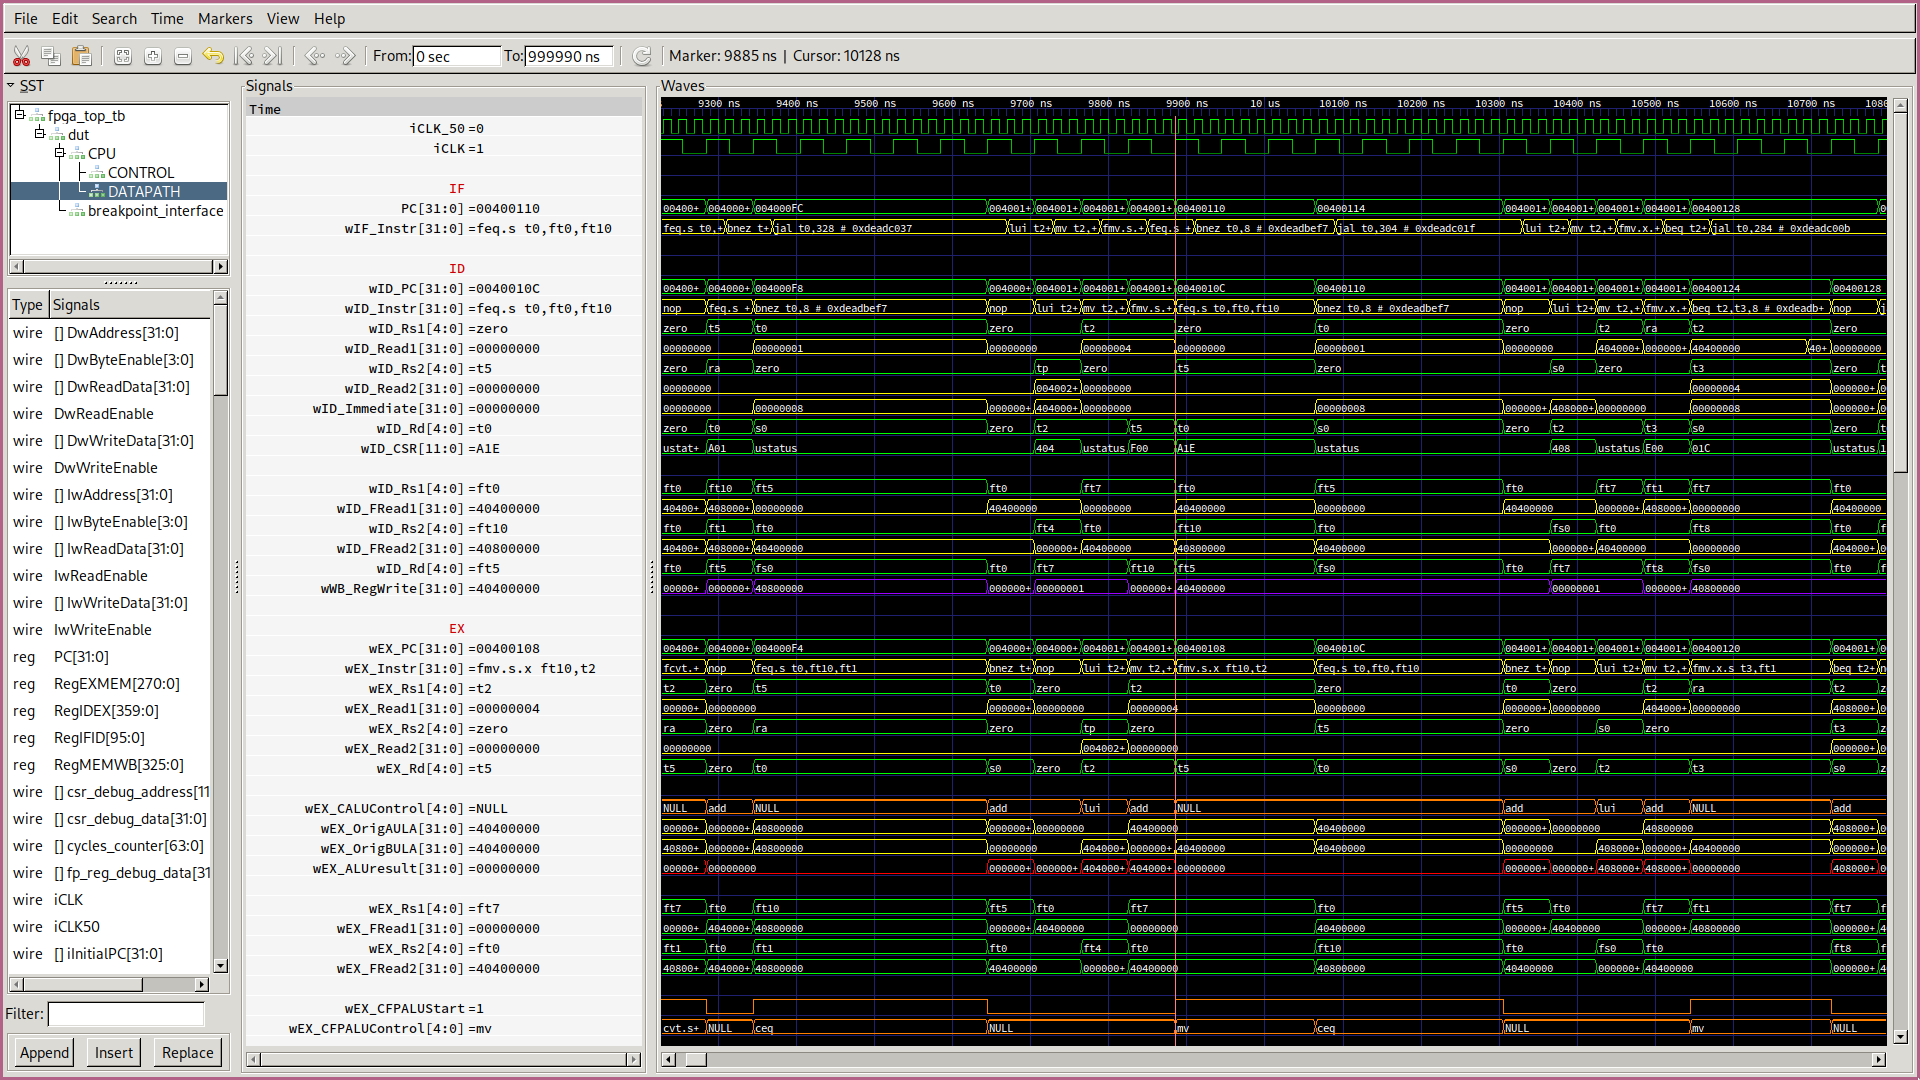
\includegraphics[width=.9\linewidth]{../images/gtkwave/random.png}
        \caption{Visualização das formas de onda no GTKWave}
        \label{fig:gtkwave_generic}
    \end{figure}

    { É possível escolher as cores dos sinais para melhor destaque, bem como
        utilizar arquivos e programas para a tradução de valores dos sinais.
        Na pasta \texttt{test/gtkwave/translation\_files} se encontram arquivos
        \texttt{.txt} para tradução dos códigos hexadecimais dos seletores de
        registradores e de controle das unidades de lógica e aritmética. Assim,
        a visualização da forma de onda mostra os mnemônicos dos sinais, facilitando
        sua compreensão. O programa \texttt{riscv-decode} presente em
        \texttt{tools/riscv-disassembler/build} desmonta as instruções e as exibe
        na visualização.
    }


\section{Script \texttt{make.sh}}
    { A pasta \texttt{test/sof\_library} contém os arquivos \texttt{.sof} com
        as nove variações da última versão do processador, prontos para serem
        gravados na \textit{FPGA}. Para facilitar a geração das nove variantes,
        o \textit{bash script} \texttt{make.sh} foi criado para automatizar a
        síntese, salvando as novas versões na pasta \texttt{test/sof\_library}.
        O \textit{script} também permite realizar somente a etapa de
        análise das variantes para confirmar que alterações feitas no código não
        introduziram erros de compilação, uma vez que é um processo muito mais
        ágil que realizar a síntese completa.
    }

    { Além disso, o \textit{script} também possui opção para simular \textit{RTL}
        todas as variantes do processador, salvando os \textit{logs} e arquivos
        \textit{.vcd} na pasta \texttt{test/simulation}. A pasta \texttt{test/simulation}
        é ignorada pelo \textit{git}, pois os arquivos de forma de onda podem
        ficar grandes demais a ponto de inviabilizar seu versionamento.
    }

    \section{Uso da FPGA DE1-SoC}
    { A placa de desenvolvimento \textit{terasIC DE1-SoC} utilizada no projeto
        é mostrada na Figura~\ref{fig:de1_soc}.
    }

    \begin{figure}[H]
    \centering
        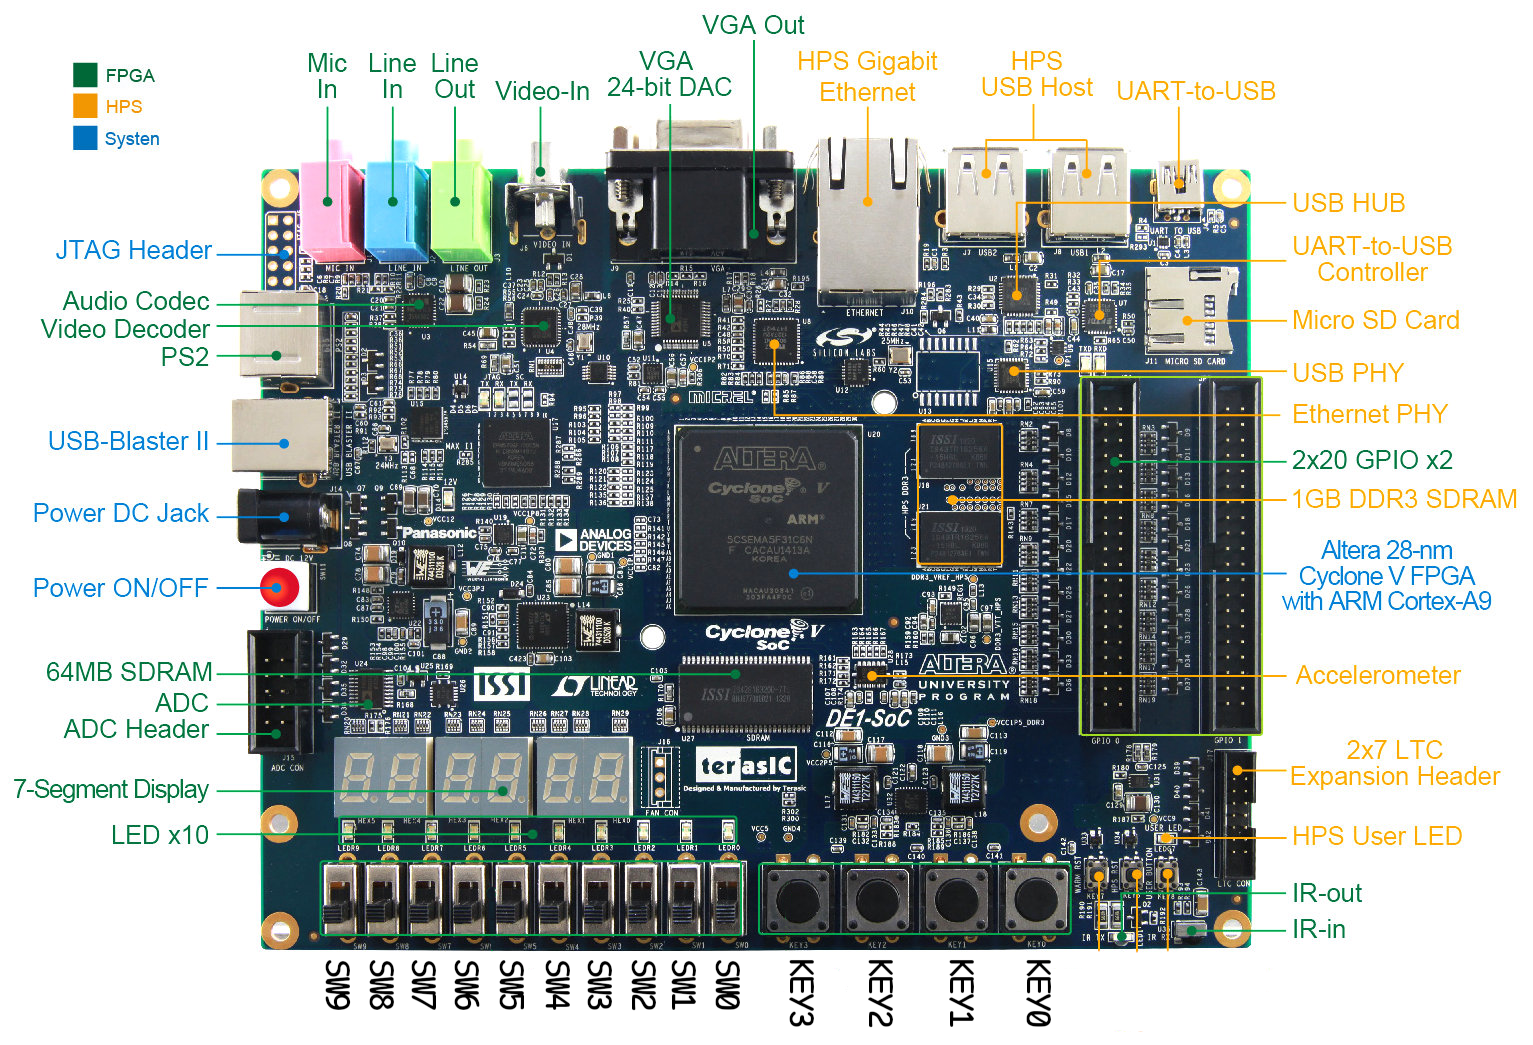
\includegraphics[width=.9\linewidth]{../images/fpga/de1_soc_subs.png}
        \caption[Placa de desenvolvimento \textit{terasIC DE1-SoC}.]{Placa de
        desenvolvimento \textit{terasIC DE1-SoC}.\quad Fonte:~\cite{terasic_de1_soc}}
        \label{fig:de1_soc}
    \end{figure}

    { Os botões e \textit{switches} mostrados na Figura~\ref{fig:de1_soc} são
        utilizados para controlar as características do \textit{clock} do
        processador, fazer seu \textit{reset} e controlar o \textit{menu OSD}
        de depuração. A função de cada \textit{input} é:
    }
    \begin{itemize}
        \item \texttt{KEY0}: Reset do processador;
        \item \texttt{KEY1}: Seletor de divisor de \textit{clock} lento ou rápido;
        \item \texttt{KEY2}: Seletor de \textit{clock} manual ou automático;
        \item \texttt{KEY3}: Gerador de \textit{clock} manual;
        \item \texttt{SW0}: Bit [0] do divisor de \textit{clock};
        \item \texttt{SW1}: Bit [1] do divisor de \textit{clock};
        \item \texttt{SW2}: Bit [2] do divisor de \textit{clock};
        \item \texttt{SW3}: Bit [3] do divisor de \textit{clock};
        \item \texttt{SW4}: Bit [4] do divisor de \textit{clock};
        \item \texttt{SW5}: Temporizador para \textit{stall} do processador;
        \item \texttt{SW6}: Seletor de \textit{framebuffer} a ser exibido;
        \item \texttt{SW7}: Seletor de banco de registradores no \textit{menu OSD};
        \item \texttt{SW8}: Sem função;
        \item \texttt{SW9}: Habilita o \textit{menu OSD};
    \end{itemize}

    { O procedimento recomendado para inicialização do processador após o
        \textit{Programmer} do \textit{Quartus} programar a \textit{FPGA} com
        um novo arquivo \textit{.mif} é: Pressionar e soltar a \texttt{KEY2}
        para ativar o \textit{clock} automático; pressionar e soltar a
        \texttt{KEY0} para dar o \textit{reset} dos estados do processador e,
        caso queira uma execução mais rápida, pressionar e soltar a \texttt{KEY1}
        para mudar para um divisor de \textit{clock} mais veloz. A frequência
        máxima de operação do \textit{clock} é de 50MHz, e ocorre na opção de
        divisor rápido com o divisor \texttt{5'b1}.
    }

    { Utilizando a saída de vídeo, o sistema pode executar programas gráficos
        como jogos, ou pode ser usado simplesmente como ferramenta de \textit{debug}.
        Ativando o \textit{menu OSD} e utilizando o \textit{clock} manual, é
        possível ver a progressão dos registradores do processador instrução por
        instrução.
    }

    { O processador também pode receber \textit{inputs} do usuário utilizando
        um teclado \textit{PS/2}. A leitura do teclado é realizada por meio de
        \textit{polling} do endereço do \textit{buffer} do teclado.
    }

    { A interface \textit{RS-232} também pode ser utilizada para enviar e receber
        dados provenientes de outro computador, permitindo contornar a limitação
        de pouca memória disponível na \textit{FPGA}, enviando novos dados e
        instruções à medida em que forem necessários e/ou requisitados pelo
        processador.
    }


\section{Observações finais do sistema proposto}
    { No presente capítulo vimos o detalhamento da implementação e das ferramentas
        utilizadas no ambiente de aprendizado, e como utilizá-las. No próximo
        capítulo, trataremos dos resultados do trabalho, apresentando tabelas
        comparativas entre as implementações, análise de performance e visualizações
        das formas de onda do sistema simulado.
    }

